\documentclass[a4paper, twoside, 12pt]{report}

%% Language and font encodings
\usepackage[english]{babel}
\usepackage[utf8x]{inputenc}
\usepackage[T1]{fontenc}

%% Sets page size and margins
\usepackage[a4paper,top=2cm,bottom=2cm,left=3cm,right=3cm,marginparwidth=1.75cm]{geometry}
%top was 3cm

%% Useful packages
\usepackage{amsmath}
\usepackage{amsfonts}
\usepackage{graphicx}
\usepackage{tabularx}
\usepackage{adjustbox}
\usepackage[table]{xcolor}
\usepackage{wrapfig}
\usepackage{caption}
\usepackage{subcaption}
\usepackage[colorinlistoftodos]{todonotes}
\usepackage[colorlinks=true, allcolors=blue]{hyperref}
\usepackage[numbers]{natbib}

\usepackage{algorithm}
\usepackage[noEnd=false, indLines=false, spaceRequire=true, beginComment=//~]{algpseudocodex}
\renewcommand{\algorithmicrequire}{\textbf{Input:}}
\renewcommand{\algorithmicensure}{\textbf{Assert:}}

% load some macros
\newcommand{\speech}[1]{``#1''}
\newcommand{\socalled}[1]{`#1'}

\newcommand{\reffig}[1]{Figure \ref{#1}}
\newcommand{\refchap}[1]{Chapter \ref{#1}}
\newcommand{\refsec}[1]{Section \ref{#1}}
\newcommand{\refsubsec}[1]{Subsection \ref{#1}}
\newcommand{\refapx}[1]{Appendix \ref{#1}}
\newcommand{\reftab}[1]{Table \ref{#1}}
\newcommand{\refalg}[1]{Algorithm \ref{#1}}

\newcommand{\pass}{Task Succeeded}
\newcommand{\fail}{Task Failed}
\newcommand{\er}[1]{$\theta$=#1}


\DeclareMathOperator{\derivone}{\frac{dy}{dx}}
\DeclareMathOperator{\rarrow}{\rightarrow}
\DeclareMathOperator{\darrow}{\leftrightarrow}
\DeclareMathOperator{\rArrow}{\Rightarrow}
\DeclareMathOperator{\dArrow}{\Leftrightarrow}
\DeclareMathOperator{\real}{\mathbb{R}}
\DeclareMathOperator{\nat}{\mathbb{N}}
\DeclareMathOperator{\integer}{\mathbb{Z}}
\DeclareMathOperator{\quat}{\mathbb{H}}
\DeclareMathOperator{\reward}{\mathcal{R}}
\DeclareMathOperator{\state}{\mathcal{S}}
\DeclareMathOperator{\action}{\mathcal{A}}
\DeclareMathOperator{\degrees}{^{\circ}}
\DeclareMathOperator{\qi}{\mathit{i}}
\DeclareMathOperator{\qj}{\mathit{j}}
\DeclareMathOperator{\qk}{\mathit{k}}
\DeclareMathOperator{\shortspace}{\: \: \: \:}
\DeclareMathOperator{\longspace}{\shortspace \shortspace}

\title{Lightweight One-shot Imitation Learning}
\author{Alfie Chenery}
% Update supervisor and other title stuff in title/title.tex

\begin{document}
\begin{titlepage}

\newcommand{\HRule}{\rule{\linewidth}{0.5mm}} % Defines a new command for the horizontal lines, change thickness here

%----------------------------------------------------------------------------------------
%	LOGO SECTION
%----------------------------------------------------------------------------------------


\includegraphics[width=8cm]{title/logo.eps}\\[1cm] % Include a department/university logo - this will require the graphicx package
 
%----------------------------------------------------------------------------------------

\center % Center everything on the page

%----------------------------------------------------------------------------------------
%	HEADING SECTIONS
%----------------------------------------------------------------------------------------

\textsc{\LARGE MEng Final Year Project}\\[1.5cm] % Name of your university/college
\textsc{\Large Imperial College London}\\[0.5cm] % Major heading such as course name
\textsc{\large Department of Computing}\\[0.5cm] % Minor heading such as course title

%----------------------------------------------------------------------------------------
%	TITLE SECTION
%----------------------------------------------------------------------------------------
\makeatletter
\HRule \\[0.4cm]
{ \huge \bfseries \@title}\\[0.4cm] % Title of your document
\HRule \\[1.5cm]
 
%----------------------------------------------------------------------------------------
%	AUTHOR SECTION
%----------------------------------------------------------------------------------------

\begin{minipage}{0.4\textwidth}
\begin{flushleft} \large
\emph{Author:}\\
\@author
\end{flushleft}
\end{minipage}
~
\begin{minipage}{0.4\textwidth}
\begin{flushright} \large
\emph{Supervisor:} \\
Dr. Edward Johns \\[1.2em] % Supervisor's Name
\emph{Second Marker:} \\
Dr. Pancham Shukla % second marker's name
\end{flushright}
\end{minipage}\\[2cm]
\makeatother

% If you don't want a supervisor, uncomment the two lines below and remove the section above
%\Large \emph{Author:}\\
%John \textsc{Smith}\\[3cm] % Your name

%----------------------------------------------------------------------------------------
%	DATE SECTION
%----------------------------------------------------------------------------------------

{\large \today}\\[2cm] % Date, change the \today to a set date if you want to be precise

\vfill % Fill the rest of the page with whitespace

\end{titlepage}

%TODO
\begin{abstract}
One-shot imitation learning is a leading approach in robotic learning, valued for minimizing the need for time consuming, human-collected demonstrations. However, the computational demands of these algorithms are substantial. What options exist when these requirements surpass available hardware capabilities? This paper explores alternatives to state-of-the-art one-shot imitation learning algorithms and presents a system achieving comparable results with drastically reduced hardware requirements. This advancement lowers the barrier of entry, making such systems accessible to a wider audience, without the need for high-end GPUs.

%At a time where Moore's law appears to have begun to plateau, we can no longer simply rely on new hardware to be more powerful and speed up our algorithms.\\
%In the field of robotic learning, one-shot imitation learning stands as one of the best algorithms due to its ability to reduce the workload of engineers collecting demonstrations. Instead this workload is offloaded to the algorithm, which resultantly needs huge computational power to work. But what do we do when the algorithm requirements exceed that of our available hardware? In this paper we explore alternatives to current state of the art one-shot imitation learning algorithms, and create a system which can achieve comparable results, with drastically lower hardware requirements. This lowers the barrier to entry for such systems, allowing them to be run by more people, without top of the line GPUs. 
\end{abstract}

%TODO
\renewcommand{\abstractname}{Acknowledgements}
\begin{abstract}
Firstly, I would like to thank my supervisor, Dr.~Edward Johns, for his support and guidance throughout this project. His expertise and feedback have been greatly appreciated.
\\

I would like to personally thank my sayang, Dayana Muhd Faisal, for her help proof reading and her unending support through all the challenges of this year and those previous. I would likely not be at this point without her.
\\

Lastly, I would like to thank my friends and family for their support throughout my whole degree. 
\end{abstract}

\tableofcontents
%\listoffigures
%\listoftables

\chapter{Introduction}
\label{chap:introduction}

Robotic manipulation is a complicated problem in the field of robotics in which we want a robot to interact with and influence it's environment in a specific way to complete a task. This is much more complicated than simple robot locomotion, as we don't just want the robot to move and exist within in its environment, but instead we want the robot to have meaningful interactions with certain objects in the environment. These interactions may be complex involving many moving parts, or multiple individual objects entirely. Furthermore, these interactions may be unpredictable if the robot's actions are prone to failure, or if the robot is interacting with objects it has no prior knowledge of.\\

As currently described, this problem is not particularly hard to solve. One could spend a few hours hand crafting an exact set of instructions for the robot to complete, such that when run from start to finish the robot completes the task. However, this implementation is missing a crucial feature. It does not generalise to different environments. We want the robot to be able to complete the task even when the task is placed in a different environment. Specifically the robot should be able to analyse the state of the environment prior to or during the execution of the task and be able to adapt to this environment in order to complete the task.\\

Suppose we have a robot arm in which we can control the angle of each joint and an environment which contains a coffee mug. We could easily define the exact joint angles at each time step, such that when the robot executes these positions, it manages to pick up the mug. However, if we now change the environment, and move the mug to the side, then the robot is going to fail the task. It will follow the instructions as before, trying to pick up a mug that is no longer there. This control algorithm does not generalise to different environments, it is hard coded for one specific environment setup. We want a system which can sense the environment in some way, and change it's actions accordingly, making decisions based on the information from its sensors. For example seeing the mug has been moved to the side, and changing the joint angles such that it still manages to pick it up.\\

It is obvious that hard-coding the instructions for every possible task set up is intractable. The general approach to solving such a problem involves trying to teach the robot an understanding of the meaning behind the underlying task itself, abstracting it away from the environment it is performed in. For example, we do not want to teach the robot \speech{How do I pick up \textbf{\textit{this}} mug?} We want to teach it \speech{What does it mean to pick up \textbf{\textit{a}} mug?} and \speech{How do I know when I have picked up a mug?}. These success criteria questions are something we will refer back to when considering different algorithmic approaches in \refchap{chap:background}.\\

If the robot is able to comprehend this higher level notion of what it truly means to complete the task, without relying on environment specific information, then we have successfully extracted the task out from the environment. In this sense the task can be placed in any environment, and the concept of the task itself has not changed. The robot knows how to pick up a mug in whichever environment it is found in. The robot does not need to work out how to complete the task, it only needs to compute how to apply the already known task in this new unseen environment.\\

Some existing solutions to this problem \cite{rl, rl-intro-book, inverse-rl, behavioural-cloning, rl-book, behavioural-cloning-book} offload the work of extracting environment agnostic task information to the engineers. This requires us to formalise the task in a complicated mathematical expression which can be applied to any environment. This approach, called \socalled{Reinforcement Learning}, is detailed in \refsec{sec:reinforcement-learning}. Alternatively, engineers can directly generalise the task by presenting it in many different environments and demonstrating to the robot how to complete the task in each case. This however still multiplies the workload of engineers providing large amounts of training data to the system. This method, called \socalled{Imitation Learning}, is explored in \refsec{sec:imitation-learning}. \\

Newer state of the art solutions \cite{coarse-to-fine, one-shot-pose-estimate, one-shot-imitation} build on the ideas of Imitation Learning, but instead of offloading the work to the engineers, attempt to offload the work to an Artificially Intelligent system. A common approach among these solutions is to capture specialised additional information during training time which allows the task to easily generalise. This additional information, often in the form of images taken by the robot, is something which can be automatically collected with no extra effort from the engineers. In order to process and incorporate the additional information, these papers unanimously opt to rely on Artificial Intelligence models. Either training neural networks from scratch, or incorporating pre-trained vision transformer models. In doing so these solutions achieve a remarkable feat, in that a single human provided demonstration is sufficient to learn a task which generalises to unseen environments. We explore these \socalled{One-shot Imitation Learning} approaches further in \refsubsec{subsec:one-shot}. \reffig{fig:intro} illustrates the problem we aim to solve.\\

\begin{figure}[h]
    \centering
    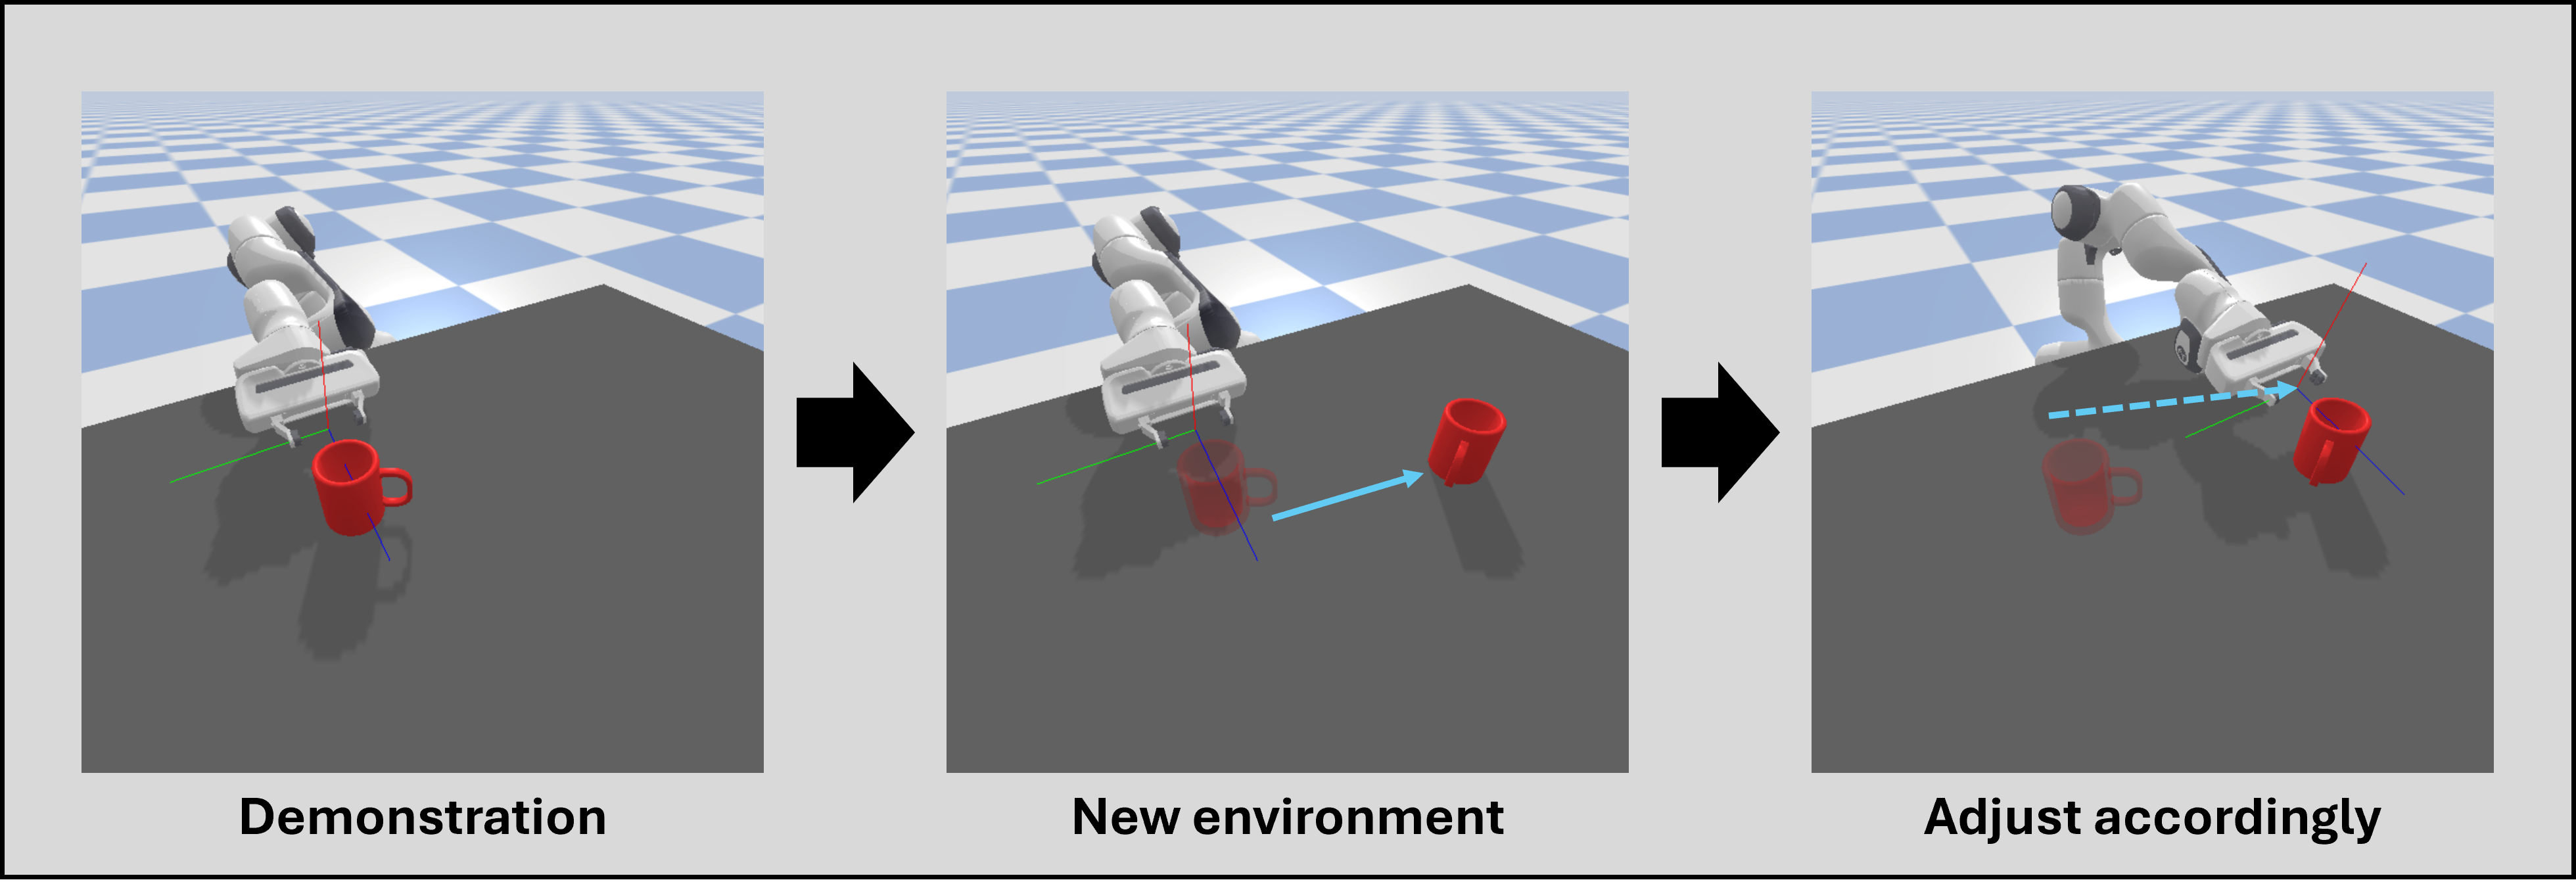
\includegraphics[width=\textwidth]{figures/intro.png}
    \caption{The One-shot Imitation Learning Problem}
    \label{fig:intro}
\end{figure}

\section{Contributions}
In this paper we consider the limitations of the aforementioned state of the art solutions. In particular we focus on \speech{DINOBot: Robot Manipulation via Retrieval and Alignment with Vision Foundation Models}, a system created by N. Di Palo and E. Johns \cite{one-shot-imitation} as a case study. N. Di Palo and E. Johns generously publicise their source code for installing and utilising the vision transformer at the heart of their system.\\

Upon implementing this system it becomes apparent that the physical hardware requirements of this and many other state of the art solutions are immense. The DINObot system requires in excess of 16GB of GPU video RAM. We are unable to find an exact requirement, since this has already reached the maximum hardware specifications of the machines available to us for this project. As such we were not able to implement the DINObot system at any point during this project. This unfortunately limits our ability to directly compare our solution to DINObot, since we cannot test DINObot on the same test suite we use to evaluate our own system. However it does highlight this issue, existing solutions are not accessible to a large portion of potential users.\\

The driving motivation for this paper is to emulate the methods of state of the art systems, to produce high quality and accurate results while operating under much tighter computational constraints. Our framework should be capable of learning tasks and generalising to novel environments from a single human provided demonstration. It should achieve this with substantially lower memory requirements, while not impacting performance and accuracy.\\

This paper manages to achieve a such a system which we call \socalled{LiteBot} in reference to its lightweight hardware requirements. LiteBot achieves comparable performance to existing solutions. One of the most significant features of the system presented in this paper is its ability to operate entirely on a CPU. The system performs efficiently without any GPU resources being utilised. Despite this LiteBot is still fast enough for real time inference during testing. Our method combines strategies from existing One-shot Imitation Learning systems, while exchanging memory intensive Artificial Intelligence components for classical algorithms from the field of computer vision. While this may seem irrelevant in an application which already requires specialised robotics hardware, the methods described in this paper have broader applications in simulations, video games and pure mathematical settings. In such fields the reduced barrier to entry becomes highly desirable. Furthermore, as shown in this paper, physical robotics hardware has become a luxury as opposed to a necessity, with high quality simulation software providing a solid basis to perform robot learning within.\\

Moreover, we create a framework which can learn multiple tasks independently. The robot is able to identify which task to complete from its corpus of trained tasks, using only observations of the environment it finds itself in and no external input from a human. It can identify the task to complete by analysing the environment, and then executes this task in the specific test time environment. It achieves all of this with minimal pre-training, each learned task consisting of a single human provided demonstration combined with automatically collected data which facilitates the generalisation to novel environments. This data comes with no additional workload to the demonstrator.\\

\section{Ethical Considerations}
This project does not work directly with people or animals. However, there could be safety considerations if deploying to a physical robot arm. These potential safety concerns are a consequence of using any robot arm and are not specific to this project. As such normal safety protocol in remaining clear of the robot arm during operation would be sufficient.\\

There are no legal or licensing concerns with this project. All libraries used are open source and can be installed through the default Python package manager, pip.\\

A widely generalisable learning agent will be applicable to many scenarios and tasks, some of which may be malicious in nature. While it is possible that work from this project could be taken and misused to teach a robot morally questionable tasks, this is not the intended use or focus of this project.\\

Finally while this project does not directly focus on environmental issues, we should consider the energy used running the simulations and equipment. While this is a non-zero amount, it is for the purposes of research and well within reasonable limits. Furthermore, this paper specifically focuses on producing a robot learning algorithm with lower hardware requirements to run effectively. This allows our system to run on lower power and more efficient machines than previously possible. While this is undoubtedly a benefit of the solution presented, reducing the environmental impacts is not the focus of this paper.
\chapter{Background}
\label{chap:background}

As discussed in Chapter \ref{chap:introduction}, a simple robot learning algorithm will allow the agent to generalise to different environment setups.
There are three main techniques which allow us to achieve this, however each of these methods come with some major drawbacks which will be discussed.

\section{Model Based Control}
\label{sec:model-based-control}
In this first method, in order to teach the robot how to complete the desired task, the human needs to provide to the robot a model of the environment and a reward function \cite{model-based-control}. The model is a function which encapsulates the dynamics of the environment, and the ways that actions influence the state. Specifically, it is a map from the current state and chosen action to the resulting next state:
$$\mathcal{P} : \state \times \action \mapsto \state$$

The reward function is some function which maps the current world state and action chosen by the agent to a real number:
$$\reward : \state \times \action \mapsto \real$$

Here $\state$ denotes the set of all possible states the system can be in, and $\action$ denotes the set of all possible actions the robot may take.\\

The robot then tries its best to maximise this reward by choosing the actions which give a high reward now, but that also lead to states with the potential to yield high rewards later. It is able to predict which states it will reach later using the environment model. The priority between getting an immediate reward now and ensuring higher rewards later is controlled through the discount factor $\gamma \in [0,1]$. If the robot is provided with these aspects, and the model perfectly captures the environment dynamics , then the robot can directly solve the induced Markov Decision Process (MDP), for example using a dynamic programming approach to calculate the expected rewards of being in every state \cite{rl-intro-book}. Then the agent can simply take the actions which ensures it follows the sequence of states with highest expected rewards.\\
%TODO: cite , dynamic programming, bellman equations

Referring back to the success criteria questions mentioned in \refchap{chap:introduction}, this method teaches the robot \speech{How do I know when I have completed the task?} The task is completed when this given reward function is maximised. It is up to the engineer to ensure that this reward function really does capture the specifics of the underlying task, since the robot has no true understanding of the task. The robot is merely trying to maximise a number, wherein it has been told that getting the number as big as possible, will complete the task. We have also implicitly defined \speech{What does it mean to complete the task?} To complete the task is to score highly in the reward function.\\

The problem with this method is it is a lot of work to design the reward function and environment model. In some cases the environment may not even be fully observable. As such a complete model is simply not possible. As a result Model based control is most often used in specific lab settings where the environment can be meticulously controlled. It is rarely used in so called \socalled{in the wild} robot learning due to the inability to guarantee control over the environment, resulting in an unreliable environment model. As such, Model Based Control lacks the generalisability we strive for in this paper, and so will not be considered further.

\section{Reinforcement Learning}
\label{sec:reinforcement-learning}
The second method at our disposal is Reinforcement Learning \cite{rl}. In this method we do not need to provide the agent a model of the environment. However, the agent still requires a reward function. The robot will explore the environment on its own to experience states and see which ones yield high rewards \cite{rl-intro-book, rl-book}. After sufficiently long training, the robot's ideas of which states have a high associated reward should approach the true values. These values were known outright in Model Based Control thanks to the environment model, however in Reinforcement Learning the agent explores the state space itself to approximate these values. The robot is then able to select the actions which lead to states it has experienced giving high rewards.\\

This method answers the success criteria questions in exactly the same way as with Model Based Control. The reward function still solely encodes information as to the completion of the task. The only difference is in how much information the robot has available to pursue improving the reward function, and hence completing the task. Instead of a perfect understanding of the world and how these interactions affect the reward function, the robot only has information it has experienced itself.\\

While this method is a big improvement over model based control, there is still a problem. We still need to provide the agent a reward function. This can be difficult to formulate, even more so without the environment knowledge of model based control. When we had access to the environment model we had knowledge of the relative positions of objects, and could easily define tasks which involved moving one object to another place. For example the reward function could be the negation of the distance between the object's position and the target position. Alas, without the environment model, the agent cannot know perfectly the position of the objects and the target position. These must be estimated from the environment observations it makes. Such observations are usually in the form of a camera attached to the robot, often mounted in a fixed third person view, or mounted on the wrist for a first person view. From these observations, the robot can estimate the position of objects, given their position in the image, and the known position of the camera when the image was taken.\\

Despite only having access to estimates through observations, carefully designing a reward function is a reasonable approach. The issue comes with the increased workload of a generalisable system. If we wish to teach the agent multiple tasks we are required to provide the agent one reward function for every task we wish it to complete. Furthermore, we need some way to decide which task to complete and select the correct reward function. Since each task may be wildly different, it is simply not possible to encode all of these tasks with a single reward function. As such, Reinforcement Learning is more applicable to fine tuning a solution to a specific task. Since the robot explores the environment itself, there is little bias to the solution, given the robot explores sufficiently within the state space. This is desirable for finding optimal solutions to a problem that the engineers may not have considered. As we will see in the next section, other solutions often introduce large amounts of human bias to the solutions the robot finds. However, poor exploration from the robot can lead to sub-optimal results, if the agent gets stuck exploiting a local optima, when it could have reached a better solution by exploring further. This tendency to get stuck with a sub-optimal solution is obviously undesirable. \\

It can be difficult to decide a strategy for this \socalled{exploration vs exploitation} problem. A high exploration means the agent can in theory experience more of the state space. However, the exploration can be very unfocused, leaving the robot exploring an area which is not likely to yield good results. Exploitation refers to the agent choosing the best action it can at its current state. A good algorithm balances some exploitation to keep the robot focused in the direction of the currently believed best solution, while allowing exploration to test out close by states, which are more likely to perform well. This balance is often achieved through \socalled{epsilon-greedy exploration}, wherein $\epsilon$ is a hyperparameter probability. The agent will choose the greedy option, the best currently known action in its current state, with proportion $\epsilon$. Otherwise it will choose any other random action with probability $1-\epsilon$. When choosing the random action, all actions are drawn from a uniform distribution. Choosing a good value for this hyperparameter is difficult and largely dependent on the specific problem environment. Additionally, this all assumes the environment is continuous, meaning that near by states behave similarly to their neighbours. If this is not the case, then keeping the exploration focused about the current optimal solution, offers little benefit.

\section{Imitation Learning}
\label{sec:imitation-learning}
With these issues in mind, the third common robot learning method is Imitation Learning. This method attempts to simplify the data collection required of the engineers and reduce the impact of hyperparameters. Instead of needing to provide a reward function to the agent, we instead provide demonstrations of how to complete the task. The key paradigm shift is that rather than telling the robot what we want it to do (through the reward function) and leaving it to work out how to do that, we instead show the robot exactly how to perform a task. This generally gives a much faster return on investment since the robot is immediately able to perform the task somewhat well, as opposed to learning an optimal solution through time consuming exploration in the environment. This does however, have a few downsides. Most notably we, the engineers, need to be able to perform the task ourselves. We cannot teach the robot to perform a task if we fail to show it a successful demonstration. Furthermore, the robot's solutions are heavily biased towards the human demonstrations. The agent will not do much exploring and innovating on the solutions presented by the humans. Depending on the implementation the agent may process the provided demonstrations differently.

\subsubsection{Inverse Reinforcement Learning}
One approach is to use Inverse Reinforcement Learning to infer the reward function from the provided demonstrations \cite{inverse-rl}. We may use a function approximator, such as a neural network to replace the reward function. Given the robot's state and chosen action, we want the approximator to output the reward for this action. In this scenario we use the demonstrations, along with associated, presumably high rewards to train this network. For example, stating that all human demonstrations receive a fixed reward of 100, since they accomplish the task. With a reward function now known, the agent can use the previously discussed forward Reinforcement Learning to solve the task in similar situations.\\

In this implementation we attempt to again teach the robot \speech{How do I know when I have completed the task?} The difference being how we convey this to the agent. We give the robot a number of demonstrations which are considered as successful completions of the task. From this the robot tries to infer what was common about all these demonstrations which makes them successful at completing the task. The difficulty lies in the fact that often very many reward functions could explain the behaviour. Was the task to grasp the mug or to just move the end effector to the right? To us it may seem obvious that it was probably the first option, but to the robot both of these options are valid.

\subsubsection{Behavioural Cloning}
Another approach is to forgo the reward function entirely. In Behavioural Cloning \cite{behavioural-cloning, behavioural-cloning-book}, the agent instead uses the demonstrations as a blueprint to follow. Similar to Inverse Reinforcement Learning, we will still train a function approximator. However this time we will be using it as the robot's policy, not the reward function. The approximator will take in the robot's current state (or an observation of the state if it is not fully observable), and predict the optimal action. This approximator is trained on the demonstrations so that for each state in the demonstration, the ground truth output is the action which the human took in the demonstration.\\

In this implementation we are changing how we answer the success criteria questions. This time we are directly teaching the robot \speech{What does it mean to complete the task?} We are teaching the robot exactly how we as humans would solve this task. In this method the robot never gets an answer to the question \speech{How do I know when I have completed the task?} The robot has no actual concept of what it is doing and how to know when it succeeds. All it knows is \speech{This is what the human did, so I should do that too.} It trusts that the demonstrations it has been given, will allow it to complete the task.

\subsection{Training data problem}
Both of these approaches to Imitation Learning require a large diverse set of demonstrations. This is because we use the demonstrations to train a neural network. As such we need lots of training data in order to expect the function approximators to produce reasonable results. The trade off is that instead of providing a single but complicated and hard to craft reward function, we instead need to supply many simple to collect demonstrations. Although note that simple does not necessarily imply easy. While the collection of demonstrations can be straight forward, either through teleoperation (remote controlling the robot) or kinesthetic demonstration (physically moving the robot yourself), we need to provide a large amount of them which can be time consuming.\\

The additional complexity of providing demonstrations is hidden in the fact that for the agent to learn effectively, the demonstrations must be of high quality. For example, we need to ensure the demonstrations actually accomplish the goal, otherwise the robot will likely also fail to achieve the goal. Since the robot does not have a reward function, it has no way to evaluate which demonstrations were good. It instead treats all demonstrations equally, trusting that they achieve the same thing we want the robot to achieve. If a demonstration slightly misses the goal, the robot may think that this near miss state, is actually the true goal state. Problems like this one make the agent very sensitive to the initial conditions, since poor quality demonstrations may prevent it from learning anything.

\subsection{State distribution problem}
Another complication is that we need the demonstrations to be diverse so that a wide variety of states are reached. If the demonstrations do not sufficiently cover the state space the robot will be operating in, then the robot will likely find itself in a state for which it has no information how to proceed. In this scenario it is likely to perform an action which seems random. This is simply because function approximators struggle to extrapolate to inputs which are out of distribution. If we want our agent to know what to do in a wide variety of states it may find itself in, then we need to show it how to handle these states, by making sure our demonstrations at some point visit these states.\\

Ensuring the demonstrations cover the state space the robot will be experiencing during testing is a difficult problem. Simply because we cannot know for sure which states the robot will need to traverse in order to reach the goal. While providing a diverse set of demonstrations is a good start, it is always possible the robot will find itself in a state for which it does not know how to proceed. \socalled{DAgger} (Dataset Aggregation) is a Behavioural Cloning technique which aims to solve this problem \cite{dagger}. In this algorithm the agent determines its policy to complete the task, then for every state along this trajectory, the system requests a demonstration from the human. This demonstration shows what the human would have done to complete the task, from this state. This ensures that we provide demonstrations for states which the robot actually visits. There are two main problems with this design. Firstly, we cannot pre-collect all the demonstrations. The robot will propose a policy, and then request more training demonstrations. The agent then needs to retrain the policy on this new training data, taking more time. This means the training time is interleaved with the test time. A preferable design would allow us to collect all the demonstrations up front, and then test the agent with no further demonstrations required. The second problem is the sheer volume of required demonstrations. DAgger requires us to collect one full demonstration from every state along the proposed trajectory. This means the number of required demonstrations is dependent on the length of the trajectory. If the environment involves a continuous state space or a task involves a very long and complex trajectory, then this increases the demonstration burden even further.\\

Alternatively, rather than requesting a demonstration for every state along the trajectory, we can instead request a demonstration only when the robot is unsure what it should do. This is a strategy employed by \socalled{Uncertainty-Based Imitation Learning} \cite{uncertainty-il}. While this still has the issue of mixing the testing and training time, it requires far less demonstrations overall than DAgger. We may use any method of quantifying uncertainty within the robot's actions. One such approach is to use an ensemble of policy networks. Each network is trained on a subset of the training data, and when the predictions of optimal action differ wildly between each network, it means the agent is unsure what to do.

\subsection{Reducing the dependency on demonstrations}
\label{subsec:one-shot}
While these previously stated methods help to ensure the demonstrations are diverse, they achieve this by collecting far more demonstrations overall. The requirement to collect a large set of human provided demonstrations is the main bottleneck in an Imitation Learning system as it is a time consuming process. We wish to reduce the requirement for large amounts of training data by leveraging alternative approaches to generalise the demonstrations.\\

The work of A. Mandlekar et al. \cite{mimicgen} proposes a system to upscale a small number of demonstrations into a larger set. Their system, \socalled{MimicGen}, takes as input a small number of human provided demonstrations. It then segments these demonstrations into \speech{object centric subtasks} and constructs new ones by stitching together subtasks. MimicGen also transforms the scene so that each demonstration is diverse in positioning. This system reduces the burden of collecting demonstrations since we now need to collect far fewer demonstrations and can simply up-sample to a larger dataset. In the paper they claim \speech{Image-based agent performance is comparable on 200 MimicGen demos and 200 human demos, despite MimicGen only using 10 source human demos.} This means we could collect only 10 demonstrations, up-sample to 200 using MimicGen and have the same accuracy as if we collected 200 demonstrations manually. This dramatically reduces the workload of collecting demonstrations.\\

Another approach to solve the need for a large set of demonstrations is to provide the agent with alternative information to allow it to generalise to unseen environments thus removing the need for a large dataset of demonstrations entirely. The logical progression of this idea is to reduce the demonstration burden on the engineers as far as possible. So called \socalled{one-shot} algorithms stand as the pinnacle of this design philosophy, by allowing the robot to learn a given task from only a single human provided demonstration.\\

Specifically, P. Vitiello, K. Dreczkowski and E. Johns utilise an RGB-D image of the environment before the demonstration in their paper titled \speech{One-Shot Imitation Learning: A Pose Estimation Perspective} \cite{one-shot-pose-estimate}. This paper creates a system which upon being presented with a new scene, takes a similar picture of this new environment. The system then calculates the transformation which maps the object of interest in the demonstration to its position in the new environment. For example the system may notice by comparing the two images that the object of interest has moved 10cm to the left and rotated 30 degrees clockwise about the Z axis. The agent then applies this same transformation to the robot pose in the demonstration trajectory. The effect of this is to transform the positions at each time step so that the robot will move to a position 10cm to the left with a 30 degree clockwise rotation when compared to the original demonstration. Conceptually what this does is map the demonstration from the old environment to the new one. Now that the demonstration has been mapped to the new environment, the agent can simply execute the transformed demonstration, which will complete the task. The above solution manages to drastically reduce the workload of collecting demonstrations for the imitation learning task. As the name \speech{One-shot imitation learning} suggests, only a single demonstration is required. Furthermore, the additional information required by the agent, the \speech{context vector} as this paper calls it, can be collected automatically by the agent during the demonstration with no additional human input needed.\\

N. Di Palo and E. Johns propose a similar method \cite{one-shot-imitation} which uses a wrist mounted camera as opposed to the previous solution which utilised a third person camera which captured the entire scene. The advantage of a wrist mounted camera is that the camera is moving with the end effector. This effectively makes the image captured translation and rotation invariant relative to the end effector pose. The only important information is the relative pose between the end effector and the object in the scene. The advantage of this is that we reduce the need for complicated computer vision methods for pose estimation of the objects between the two images \cite{one-shot-pose-estimate}. In the work by N. Di Palo and E. Johns, since the camera moves with the end effector, changes in the end effector position and orientation are reflected very obviously in the captured image \cite{one-shot-imitation}. This also means that the agent simply needs to line up the end effector so that the captured image is the same as the demonstration image. If this is the case then the relative position between the end effector and the object is the same as in the demonstration. As such the current position and orientation of the end effector after lining up but before starting the task, can be calculated using forward kinematics and added as an offset to the poses in the demonstration. As before, this transformed trajectory can now be executed which will execute the task as in the demonstration, but mapped into the new scene.\\

Another advantage is that a wrist mounted camera also reduces the noise within the image. A third person camera which captures the entire scene will capture all objects within the scene, even though only one may be of relevance to the task. This additional noise could cause the agent to incorrectly compute the transformation between the demonstration and current scene, and therefore fail the task. Alternatively, a wrist mounted camera will only capture the focused view around the end effector. This means that during the manipulation task, the object of interest will likely be the only object within the image. This focused view is much less susceptible to noise of other objects within the environment.\\

There are of course, as with every design decision, some drawbacks to using a wrist mounted camera. Most obviously, due to the focused view failing to capture the entire scene, it can be difficult to locate the object of interest. This means that a single image may no longer be enough as the object we are looking for may not be present in the image if the camera is pointing the wrong way. This necessitates a live feed of the wrist mounted camera as opposed to the single image capabilities of the third person camera, which is a major drawback.\\

The other large drawback is a consequence of this first one. Since a live feed of the image is now required, any objects blocking the camera will now cause a serious problem. This was not an issue with the third person camera as it could capture the entire scene and everything it needed to know before starting to execute the task. However with the wrist mounted camera, if the robot picks up an oddly shaped object which happens to block some or all of the image feed, then the robot will quite literally be executing the task blind. This is not such a problem for tasks involving a single object of interest, since it is assumed the robot can navigate the arm and line up with the demonstration image while no object is in its gripper, and therefore nothing should be blocking the camera. The real problem comes with multi-stage tasks.
Consider the task which is to pick up a spoon and place it in a mug. The demonstration would pick up the spoon from a particular position and angle relative to the spoon. It would then move to a particular position and angle relative to the mug and release the spoon from its gripper. Now suppose the agent is deployed on a new task with a slightly bigger spoon, and the spoon and mug rearranged. The agent would be able to find the spoon, move to a relative position which matches as in the demonstration, and execute the trajectory to pick up the spoon. However, since the task involves two objects, we can no longer just execute the entire demonstration from this point, since the relative position between the spoon and the mug may have changed. As such we need to partition the trajectory and line up the end effector relative to the object of interest for each segment. It is clear to see that the trajectory can be segmented every time the object of interest changes \cite{mimicgen}. This itself generally happens when the gripper closes, picking up the previous object of interest, or when the gripper opens, placing the grasped object in a position relative to the current object of interest. In this example initially the object of interest is the spoon, we move relative to the spoon and execute the segment of the demonstration which picked up the spoon. Now that the spoon is attached to the end effector, the object of interest is now the mug. We want to move to a position which is relative to the mug, the same as in the demonstration. At this point we can execute that segment of the trajectory to drop the spoon. This system works fine given that the camera is a live feed and so we can keep checking the relative position of the end effector to the object we currently care about. The issue however, comes when the object in the gripper is obstructing the view of the camera. If this slightly larger spoon is now blocking the camera, the agent will be unable to find the mug and line up relative to it. In this scenario there is nothing the robot can do. It needs the spoon in its gripper to progress to the next segment of the demonstration, but when it is holding the spoon it cannot see the environment. The robot is unable to know its location relative to the mug, so cannot progress with the next segment. This demonstrates the issue with a wrist mounted camera. There are some objects which when picked up will block the camera, and there is very little the robot can do to work around this. There are just some objects the agent cannot deal with. The affects of this issue can be mitigated by careful placement of the wrist mounted camera. Placing it further up the wrist away from the end effector makes it less prone to being blocked by the object in the gripper. While this is potentially a big problem, it is unlikely that this will happen in practice. This issue could be further prevented by utilising two cameras, perhaps one on each side of the wrist, reducing the chance that an object would block both cameras, rendering the robot blind again. Of course with all these solutions, a contrived scenario with an object shaped perfectly to block the cameras will cause problems. However with everyday regular items, the affects of this problem should be limited.\\

Having reviewed the current literature, we now cover some preliminary knowledge which will be necessary in understanding the system we develop in this paper.

\section{Preliminaries: Rotations and Orientations}
\label{sec:rotations}
Throughout this report best effort will be made to not confuse the terms \socalled{rotation} and \socalled{orientation}. While mathematically these terms are represented identically, they have different semantic interpretations. As such the language within this paper will be consistent with the following definitions:
\begin{itemize}
    \item \textbf{Rotation:} a function which refers to the circular movement of an object around a central point or axis.
    \item \textbf{Orientation:} an angular displacement relative to an agreed upon reference frame. It is the resulting state after a rotation is applied to a body which was initially in the starting reference frame. Typically the base orientation will be such that the object's local coordinate frame aligns with the world coordinate frame. The object's orientation is then the rotation about the object's local origin, which aligns the world reference frame with the object's local reference frame.
\end{itemize}

From these definitions we can realise that to find an object's new orientation following a rotation, we compose the applied rotation with the object's previous orientation. This results in the total rotation which maps the object from the base reference frame to its new local frame, which is by our definition, its new orientation.\\

\begin{figure}[h]
    \centering
    \begin{subfigure}[b]{0.45\textwidth}
        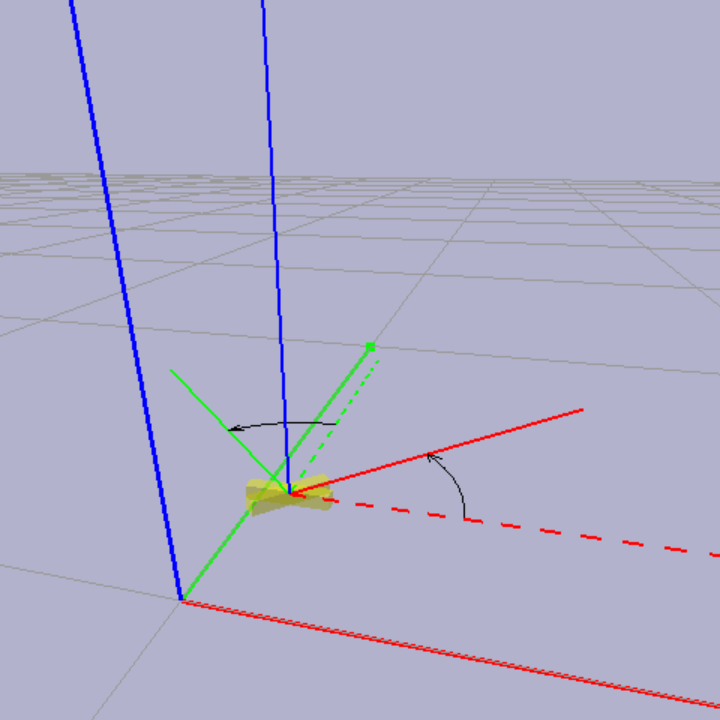
\includegraphics[width=\textwidth]{figures/coordinate_figure1.png}
    \end{subfigure}
    \hfill
    \begin{subfigure}[b]{0.45\textwidth}
        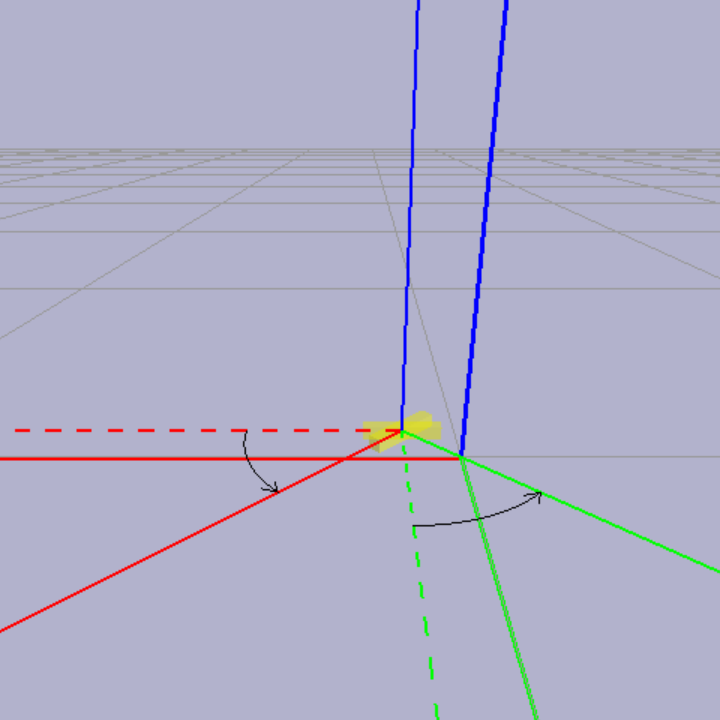
\includegraphics[width=\textwidth]{figures/coordinate_figure2.png}
    \end{subfigure}
    \caption[An object before and after a rotation of $\frac{\pi}{4}$ about the Z axis]{An object before and after a rotation of $\frac{\pi}{4}$ about the Z axis \footnotemark}
    \label{fig:orientations}
\end{figure}
\footnotetext{Refer to \refsubsec{subsec:right-hand-rule} for an explanation on rotation direction}
%TODO latex flags an error but it seems fine. Double check figure and footnote are fine before submission

\reffig{fig:orientations} showcases an object in two different possible orientations. The dotted lines show the object's local coordinate frame prior to the object being rotated. We can see that the dotted coordinate frame aligns with the world coordinate frame, just translated by the object's position. As such we define this orientation as the initial frame of reference. Therefore we would choose to encode this orientation as the identity rotation since no rotation is needed to align the world frame with the object's local frame.\\

The solid line coordinate frame shows the object's local coordinate frame after it has been rotated $\frac{\pi}{4}$ radians about the Z axis \textit{from the initial frame of reference}. Therefore we represent this orientation with the rotation $\frac{\pi}{4}$ radians about the Z axis. It would be equally valid to encode this as the rotation matrix, Euler angles or any other encoding of this rotation, but we will see in the next subsection that the method used in this project is quaternions. \reffig{fig:orientations} shows the exact same setup from two different view points, to better visualise the rotation described.

%Given this project focuses on manipulating objects in 3D space, it would be pertinent to understand the main way these rotations and orientations are encoded in our system.
\subsection{Quaternions}
\label{subsec:quaternions}
Quaternions are a 4 dimensional number system \cite{quaternions} which can be used to represent and manipulate orientations and rotations in 3D space \cite{orientations}. In many ways they are an extension of the complex numbers, adding an additional 2 complex axes. A quaternion consists of a real component and 3 imaginary components which are often grouped together and called the vector component.
$$q \in \quat, \longspace q = a + b\qi + c\qj + d\qk, \longspace where \: \: a,b,c,d \in \real$$
The fundamental imaginary units follow the set of rules listed below:
\begin{itemize}
    \item $\qi \neq \qj \neq \qk$
    \item $\qi^2 = \qj^2 = \qk^2 = \qi\qj\qk = -1$
    \item $\qi\qj = \qk, \shortspace \qj\qi = -\qk$
    \item $\qj\qk = \qi, \shortspace \qk\qj = -\qi$
    \item $\qk\qi = \qj, \shortspace \qi\qk = -\qj$
\end{itemize}

Of relevance to us however, is how these numbers can represent 3D rotations. If we consider a rotation in axis-angle form, that is that we rotate some angle $\theta$ about some normalised unit vector $v = (x,y,z)$, then we can produce the unit quaternion:
% $$q = \cos{\frac{\theta}{2}} + x\qi \sin{\frac{\theta}{2}} + y\qj \sin{\frac{\theta}{2}} + z\qk \sin{\frac{\theta}{2}}$$
$$q = \cos{\frac{\theta}{2}} + (x\qi + y\qj + z\qk) \sin{\frac{\theta}{2}}$$
This quaternion is an encoding of the specified rotation. For the quaternion to encode a rotation with no scaling, the quaternion must be of unit length:
$$q = a + b\qi + c\qj + d\qk, \longspace |q| = \sqrt{a^2 + b^2 + c^2 + d^2} = 1$$
This property will be satisfied if $v$ is a unit vector, or can be achieved otherwise by simply normalising the quaternion, dividing each component by its L2-norm.\\

Furthermore, we know by Euler's rotation theorem \cite{euler-theorem} that for any composition of rotations to a sphere about its centre, there exists a diameter of the sphere which forms an axis, and an angle for which rotating about said axis produces the same net displacement as the composition. We can generalise this to any rigid body by considering the circumscribing sphere centered on the object's position. From this we can convince ourselves that for any orientation the object could be in, we can represent it as a single axis vector and rotation angle, which we can then encode as a quaternion.\\

Quaternion addition and multiplication mirrors that of the complex numbers. Considering the numbers as expressions and simplifying like terms. However it is important to note that unlike the complex numbers, quaternion multiplication is not commutative. Multiplying quaternions is still associative.
$$qp \neq pq, \longspace pqr = (pq)r = p(qr)$$

If q is a unit quaternion, then the inverse is the same as the conjugate, gained by negating the vector part of q, while leaving the real part unaltered.
$$ q = a + b\qi + c\qj + d\qk, \longspace |q| = 1 \implies q^{-1} = q^* = a - b\qi - c\qj - d\qk$$

A unit quaternion q which represents a 3D rotation can be used to rotate a vector in the following manner:\\
Create the pure quaternion $p$ with real component = $0$, and vector component equal to $v$. Note that $v$ does not necessarily need to be a unit vector.
$$v = [x,y,z], \longspace p = 0 + x\qi + y\qj + z\qk $$
Then the rotated vector $v'$ is given by:
$$v' = [x', y', z'] \shortspace where$$
$$p' = w' + x'\qi + y'\qj + z'\qk = qpq^{-1}$$

While this is a nice property which makes rotating vectors very computationally easy, it is not the operation we will be performing most often. As mentioned above, we consider orientations as a rotation relative to a starting reference frame. Therefore, to rotate an object, we need to compose the desired rotation quaternion, with the current orientation. If the current orientation is stored as a unit quaternion q, and we wish to rotate the object by some unit quaternion r, then the resulting orientation is given by:
$$q' = rq$$
We can see that this is the correct formula for composition of rotations by using it to rotate a vector.
$$v' = qvq^{-1}, \longspace v'' = rv'r^{-1}$$
$$\implies v'' = rqvq^{-1}r^{-1} \implies v'' = (rq)v(rq)^{-1}$$
Hence rotating $v$ by $q$ and then by $r$ is equivalent to rotating a single time by the composition rotation $rq$.\\

The other operation we make use of in this paper is calculating the rotation between two orientations. That is to say given two orientations $q$ and $q'$, we want to find the rotation $r$ such that rotating $q$ by $r$ gives $q'$. If the orientations were stored as vectors then this is a more complicated procedure. However, as discussed, we represent orientations as rotations relative to a starting reference frame. In this setup, it is obvious to see that given $q$ and $q'$ are themselves rotations we could first rotate by the inverse of $q$ to get back to the starting reference frame, followed by rotating by q'.
$$r = q'q^{-1}$$
We can verify that this satisfies our desired equation:
$$rq = (q'q^{-1})q = q'(q^{-1}q) = q'$$


\subsection{The right hand rule}
\label{subsec:right-hand-rule}
The right hand rule refers to a convention defining the positive direction for rotation about an axis. While using your right hand to make a \socalled{thumbs up pose}, your thumb represents the positive direction of the axis of rotation, and your fingers curl in the direction of positive rotation. This can be seen in \reffig{fig:right-hand-rule}.\\

\begin{figure}[h]
    \centering
    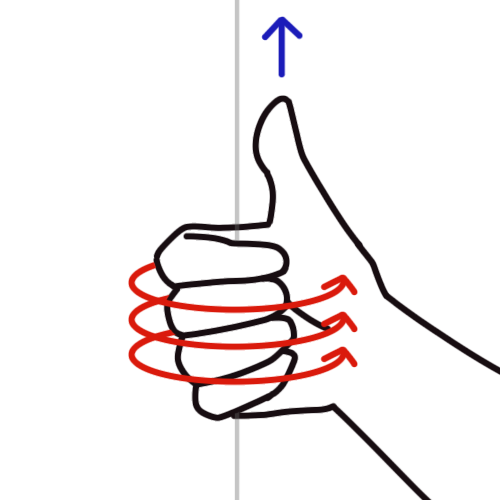
\includegraphics[width=0.7\textwidth]{figures/right-hand-rule.png}
    \caption{The right hand rule for rotation}
    \label{fig:right-hand-rule}
\end{figure}

We note that if we were to invert our hand, so that our thumb points in the opposite direction, then the fingers now curl in the opposite direction relative to the initial axis. Therefore we can imagine if we were to rotate in the negative direction about this inverted vector, we would achieve the same rotation as before. This is to say a positive rotation about some vector is equivalent to a negative rotation about the negation of the vector.\\

This is the reason that quaternions are considered a \socalled{double cover} of 3D rotations, since these two constructions describe the same rotation, but are represented by exactly 2 distinct quaternions, q and -q.
$$ q = \cos{\frac{\theta}{2}} + v\sin{\frac{\theta}{2}} \longspace and \longspace -q = -\cos{\frac{\theta}{2}} - v\sin{\frac{\theta}{2}}$$





%old stuff
%In the context of robot manipulation, reinforcement learning stands as one of the most widely used paradigms. Reinforcement learning allows for a single agent to iteratively improve at a given target task. A reinforcement learning task is characterised by 3 main factors: The set of possible states the agent and environment can be in, the set of actions which the agent is allowed to take, and the reward function which informs the agent how well it has performed.
%While these first two points are often out of our control, defined by the environment setup and the robot respectively, the third point is something problem specific which needs defining. A standard reinforcement learning agent will need a distinct reward function for each individual skill the robot wants to learn. This is a time consuming process and may not even be practical for all tasks.

%\section{Imitation reward function}
%A common solution to this problem is to define the reward function in a manner that is generalisable to other tasks. A popular example is the use of mimicry. In this case the robot is provided a demonstration, either through teleoperation or kinesthetic movement which it remembers as how to perform this skill. The reward function then becomes making the robot copy this demonstration as closely as possible. While this is a good start, if the robot only tries to copy the demonstration, the agent will not be robust to changes in the environment or slightly different problem setups. Consider a demonstration which tells the robot how to pick up a mug. If we were to test the robot by moving the mug but provided it no additional information, the robot would obviously fail to pick up the mug. This is because the robot's reward function is not encoded as \speech{Did I pick up the mug?} because this would be very difficult to formalise. Instead the robot is just asking \speech{Did I follow the demonstration?} which it did. In order to make the agent generalisable to different setups it needs more information.
%Talk about multiple demonstrations and how that method works.
%The problem with this method is that it is still time consuming and could be costly to use the equipment for multiple runs. Furthermore, this method has high variability based on the quality of the demonstrations provided. If the demonstrations are not sufficiently diverse, then the agent may struggle with some problem setups it had not encountered.

%In an attempt to alleviate some of these problems, the paper on mimicGen (reference) poses an algorithm to produce a large dataset of demonstrations from only very few human demonstrations. This drastically reduces the mount of human interaction needed. The paper claims \speech{Agent performance is comparable on 200 MimicGen demos and 200 human demos, despite MimicGen only using 10 source human demos}. What this means is that instead of needing to perform 200 human demos, you only need to perform around 10 without loss in performance. Additionally, mimicGen is specifically designed to create a diverse set of demonstrations, reducing the problem of the agent finding itself in a specific problem setup it doesnt have much information about.

%The One shot imitation papaer (reference) uses an alternative aproach to prevent needing to collect multiple demonstrations at all. Instead of collecting additional information through repeated demonstrations, it saves an image of the problem setup before the demonstration is given which it calls the \speech{context vector} This image is stored along with the single demonstration of the task. This provides the agent the context in which this demonstration was useful. In order to perform the demonstration in a new unseen problem setup, the agent first takes a picture of the new problem setup. This picture is taken using an RGB-D camera. The agent then estimates the pose transformation between the object of relevance in the demonstration image and this new image. Once the agent has estimated the transformation, it can apply this same transformation to the demonstration it was given. By doing so it transforms the demonstration into this new problem setup, wherein the agent can simple imitate the transformed trajectory to complete the task. 
\chapter{Technical Design}
\label{chap:technical}

\section{Project Scope}
By design this project aims to create a generalisable robot learning algorithm which will have applications in multiple problem scenarios. The generalisability comes from the ability to provide a robot with whatever demonstrations are relevant to solving the desired task, without requiring any changes to the core system. However, in the interest of keeping this project focused we choose to implement and analyse specifically an agent for generalised object manipulation tasks focused around grasping and moving simple objects. 
\\

\subsection{Environment specifics}
\label{subsec:pybullet-specifics}
For this project we conduct the experiments in a real time physics engine, called \socalled{PyBullet} \cite{pybullet}, available as an open source python package. As such the algorithms presented in this paper will be implemented in Python and the experimental results and evaluation will be conducted in this simulation space.\\
The specific robot arm used throughout this project is a simulation of the \socalled{Franka Panda robot arm}, which comes built in with PyBullet. This arm can be seen in \reffig{fig:arm-normal}.

\begin{figure}[h]
    \centering
    \begin{subfigure}[b]{0.45\textwidth}
        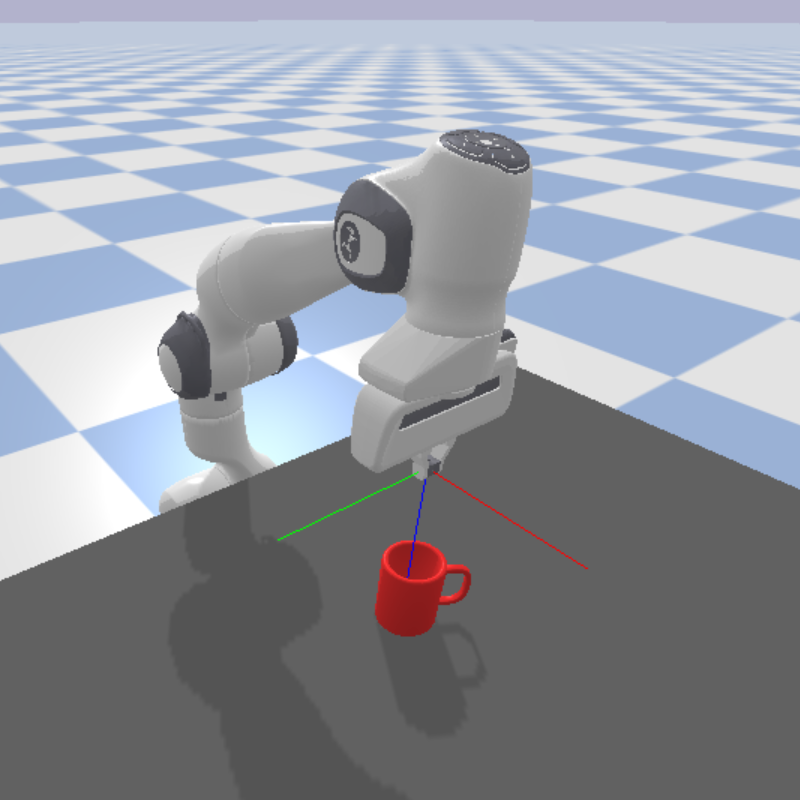
\includegraphics[width=\textwidth]{figures/robot-arm.png}
        \caption{Normal view}
        \label{fig:arm-normal}
    \end{subfigure}
    \hfill
    \begin{subfigure}[b]{0.45\textwidth}
        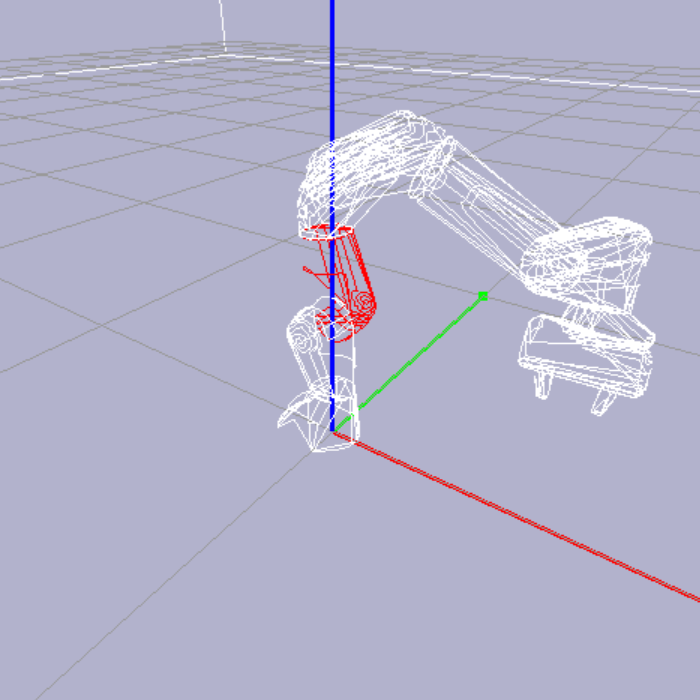
\includegraphics[width=\textwidth]{figures/robot-arm-wireframe.png}
        \caption{Wire-frame view}
        \label{fig:arm-wire}
    \end{subfigure}
    \caption{Franka panda robot arm in PyBullet simulation}
    \label{fig:robot-arm}
\end{figure}

This simulation and arm have a number of intricacies which posed a steep learning curve near the start of this project. This subsection highlights a few of these. The first major hurdle was with the accuracy of the inverse kinematics system built into Pybullet. The initial inaccuracies were not a bug in the simulation, but a misunderstanding of the signature of some of the functions.
The Franka panda robot arm has 12 individual joints. However, upon closer inspection it becomes apparent that 3 of these joints are not actuated and are fixed in place relative to the previous joint. As such the arm only has 9 degrees of freedom, while reporting all 12 joints. This issue is only apparent when using inverse kinematics to calculate the joint angles to reach a desired end effector position, since this function returns a list of length equal to the degrees of freedom of the arm. This means we get a list of 9 angles instead of 12. The function to control the arm motors, \verb|pybullet.setJointMotorControlArray()| expects one angle for every joint. As such if we pass the list of joint angles directly, we end up trying to move some of the fixed joints, while leaving the top 3 joints unspecified, resulting in not moving them. While this is not difficult to fix, there are numerous inconsistencies in the signature of different functions, which are not clearly documented. Each of these issues slowing down development while it is debugged.\\

Another point of note specific to the simulation is how cameras are implemented. The camera's in Pybullet do not use the standard intrinsic and extrinsic matrix to convert world coordinate to pixel coordinates in the image. Pybullet instead uses a projection matrix and view matrix respectively. These broadly serve the same purpose with the view matrix capturing the position and orientation of the camera and the projection matrix capturing the specifics for how points are projected onto the 2d image. The most notable difference is that the projection and view matricies are $4\times4$ instead of $3\times3$, since they consider homogeneous coordinate points. In this paper we will refer to the projection and view matrix as this is what our simulation uses. However, one could easily use a system which instead requires an intrinsic and extrinsic matrix instead.

%TODO put this somewhere
 In PyBullet, orientations are represented using quaternions, \cite{quaternions}\cite{orientations} an explanation of which is provided in \refsec{sec:rotations}. Despite adding a fourth dimension, quaternions provide a big advantage over the alternative of Euler angles. This being that quaternions do not suffer from \socalled{gimbal lock}. %TODO: cite gimbal lock

\subsection{Collecting demonstrations}
In order to generate the trajectories needed for the imitation learning system, a utility program is created to streamline the collection of demonstrations. This program generates trajectories by recording key frame poses throughout the demonstration. The demonstration can be copied by matching each of these key frame poses, with interpolation poses between them.
This program allows for the user to control and move the end effector position and orientation in Cartesian world coordinates. Once the arm is positioned in the correct pose, the user can save the current pose as a key frame of the trajectory. From here they can move the arm again and save the next key frame. If a mistake is made, the user can revert the robot arm to the last saved key frame.\\
The trajectory is stored as a list of end effector poses, the reason for which will be discussed in \refsec{sec:trajectories}.

The program is written to interface with a video game controller, so that the user can control the robot using an analogue input method such as the joysticks. This makes the program slightly more user friendly, as moving the joystick only slightly will move the joint very slowly and so allows for finer control.\\
In addition to controlling the robot, the program allows for camera rotation and zooming to better see the full robot pose, and can also enable a wire-frame view, visible in Figure \ref{fig:arm-wire}.
%TODO proof read and maybe flesh this out a little more
%TODO get new figures in table environment without joint colour coding


\section{Encoding the problem}
\label{sec:trajectories}
In this paper we plan to build upon existing ideas in the field while reducing the barrier to entry formed by using extremely resource intensive AI models. We intend to provide the robot with an example trajectory which successfully accomplishes the skill, in addition to some further context which allows the robot to generalise this trajectory to different environments. The nature of this context will be discussed further in \refsec{sec:dinobot}.\\

Let us formalise the concept of a demonstration trajectory, as this will be key in understanding how we can extract useful information from the environment it was presented in, into other unseen environments. Firstly we decompose the state of the system at time t as the current state of the robot and the state of the environment.
$$s_t = (s^{(r)}_t, s^{(e)}_t)$$

\subsection{Robot state}
We have a number of options for how to represent the state of the robot. The most expressive approach is to record the angle of every joint of the robot. This uniquely defines an exact pose of the robot.
\\
Another option to encode the robot's state is to use the end effector position and orientation. This option is appealing since for the purposes of performing manipulation tasks, the end effector pose is our main concern. We likely do not care about how the robot achieves this end effector pose, so long as it does. For this reason storing only the end effector pose at each time step, and dynamically computing the joint angles to achieve this using inverse kinematics, appears to be a desirable choice.\\

However it is worth considering that in this case an end effector pose does not uniquely define the entire robot pose. This is because the end effector pose has 3 degrees of freedom for the position and 3 for the orientation (4 quaternion components however the sum of squares must equal 1, tying down the 4th value once 3 are already chosen). In contrast the robot used in this project has 9 degrees of freedom, as discussed in \refsubsec{subsec:pybullet-specifics}. This means that the inverse kinematics system of equations is underdetermined since we have in essence 6 constraints but 9 unknowns to satisfy them with. As such, the inverse kinematics has infinitely many solutions. What this means for us is that the end effector pose does not uniquely define an entire robot pose. There are in theory infinitely many robot poses which would result in the end effector reaching the position and orientation we wanted it to.\\

\reffig{fig:underdetermined} demonstrates an analogous instance in 2 dimensions for easier viewing. In this system the target position is an (x,y) position and the orientation can be defined by a single angle. This means we have 3 degrees of freedom. Therefore, a robot arm with 4 or more controllable joints would create an underdetermined system. \reffig{fig:underdetermined} showcases just 3 possible solutions, but one can imagine how infinitely many may exist. One can also extrapolate this idea into 3 dimensions.

\begin{figure}[h]
    \centering
    \begin{subfigure}[b]{0.3\textwidth}
        \includegraphics[width=\textwidth]{example-image-a.png}
    \end{subfigure}
    \hfill
    \begin{subfigure}[b]{0.3\textwidth}
        \includegraphics[width=\textwidth]{example-image-b.png}
    \end{subfigure}
    \hfill
    \begin{subfigure}[b]{0.3\textwidth}
        \includegraphics[width=\textwidth]{example-image-c.png}
    \end{subfigure}
    \caption{An underdetermined inverse kinematics system has multiple solutions}
    \label{fig:underdetermined}
\end{figure}

While this initially seems like a big problem, for our purposes we truly do only care that the end effector is in the position and orientation we want. Any of the satisfying robot poses will do. Working with the end effector pose directly also simplifies a lot of our work later on. We will see in \refsubsec{subsec:alignment} that a lot of our calculations will involve the end effector pose. While we could compute this using forward kinematics if the demonstration instead stored joint angles, this would be an unnecessary extra step for no real benefit to the accuracy of the system. A way to use the underdetermined nature of the system to our advantage is explored further in \refappendix{apx:null-space}.\\

We may optionally decide to also include velocity information in addition to positional information. This would allow us to specify that the robot should have an exact position, but also describe how it should move in the next time step. While this may be useful for very specific tasks like throwing an object to an exact target; for the majority of tasks, velocity information is simply not necessary when we have the position for the next key frame already defined. If we were to save a key frame every time step, then the velocity information would be completely redundant, with velocity being directly computable as the displacement between the two key frames divided by the time step. In practice, for usability, we opt to not do this and only record key frames when deemed necessary by the user during the demonstration. While this does mean velocity information is not directly knowable, we decide that velocity information is not necessary for the simple tasks we are experimenting with in this paper.\\

One final thing to consider with how to represent the robot state is the gripper of the end effector. We decided to use inverse kinematics and just define the position and orientation of the end effector. However, the gripper arms are attached to the end effector. Moving the gripper arms will not affect the pose of the end effector. This means that the inverse kinematics solution will still be a valid solution whatever position the gripper arms are in. Therefore, we need to add some information to our state which uniquely decides where the gripper arms are. We could use the angle of each gripper arm, however it is unlikely we would want the grippers at different angles, so we can simplify to a single angle which we mirror for both grippers. However, we can simplify even further. We do not anticipate a situation where the gripper would need to be in an intermediate half closed state. We either want the gripper fully closed, applying a constant pressure to the item it is holding, so that the item does not fall out of its grasp, or we want the gripper fully open, so that it can drop the item it is holding. As such we can see that a single boolean value is sufficient to define the gripper state in our situation.
$$g \in \{0,1\}$$

With these decisions in place we can define the robots state as an 8 vector, containing the position and orientation of the end effector, along with the gripper state. 
$$s^{(r)} = [x_{eef}, y_{eef}, z_{eef}, a_{eef}, b_{eef}, c_{eef}, d_{eef}, g]$$

\subsection{Environment State}
We define the state of objects similarly to how we defined the end effector pose storing the 3D position and orientation of the object within the scene. Objects do not have an associated gripper, so an objects state is a 7 vector. The state of the whole environment is just the collection of all the object states within the scene.
$$s^{(e)} = \{[x_o, y_o, z_o, a_o, b_o, c_o, d_o]\}_{o=1}^O$$

We note that without a perfect model of the environment, the environment's state is not fully observable. In implementation we will not be able to capture the full environment state and instead choose to represent it differently entirely. For example capturing the environment state as an image of the scene using methods similar to those employed by P. Vitiello, K. Dreczkowski, and E. Johns \cite{one-shot-pose-estimate}. For now we will continue in the purely theoretical sense, where the environment state can be fully observed.\\

\subsection{Trajectories and Demonstrations}
Given that we have defined the state of the system, a naive approach would be to define a trajectory as the list of states traversed at each time step of the trajectory.
$$\tau = \{s_t\}_{t=1}^T$$
We can now clearly see that a trajectory is a large $T \times D$ matrix where $D$ is the dimensionality of the state. $D = 8 + 7 \cdot O$ in this idealised setting.
$$\tau \in \real^{T \times D}$$

This definition is naive for a number of reasons. Firstly we can see that a trajectory defined in this manor will include a large amount of unnecessary information. In completing a task, we will likely only need to move the robot arm to a few key positions to ensure the task succeeds. However this current definition saves a pose at every time step. We can reduce the dimensionality of a trajectory substantially if instead of saving the robot's state at every time step, we only save the relevant key frames. When executing this trajectory we will then interpolate the poses between each key frame, to recover the pose at each time step. We can now add as many key frames as are required to fully express how to complete the task, without including unnecessary in between poses. We denote a trajectory as having $K$ key frames.\\

Another issue with the current trajectory definition is that in addition to the environment state not being fully observable, it is not directly within our control. We cannot choose to change the state of the environment by magically moving an object. We can only influence the environment through the actions of the robot. As such, this approach still includes a large amount of irrelevant information. Furthermore, we want a trajectory to encode a skill. The necessary steps the robot needs to take to complete some task. This task can be completed regardless of the specific environment state and so the environment variables should not be a part of the trajectory. Conceptually, the trajectory encapsulates a skill independent of the environment it is within. The notion of influencing the trajectory based on the environment is considered more a transformation applied to the trajectory, than a component of the trajectory itself.\\

This is an important difference in definition to a demonstration. A demonstration is a human provided trajectory accompanied with some additional environment information. This additional information is what allows us to compare scenes and transform the trajectory. The trajectory itself does not include any environment specific information.\\

With these new definitions in mind we can see the trajectory is a $K \times D$ matrix where K is the number of key frame poses and $D$ is only the dimensionality of the robot's state, $D = 8$.
$$\tau = \{s^{(r)}_t\}_{k=1}^K$$

A demonstration is a trajectory combined with some environment information, which for now we denote as $\Sigma$. $\Sigma$ must correspond to the exact environment in which $\tau$ was presented by the human.
$$\Delta = [\tau, \Sigma]$$

\subsection{Environment context}
There are numerous ways we could choose to define $\Sigma$, each with their own benefits and drawbacks. The purpose of $\Sigma$ is to provide some context as to how the world looked when the trajectory was given. We will then compare this to the environment at test time, and modify the trajectory into the new scene.
$$\tau' = f(\tau, \Sigma, \Sigma')$$
Where $f$ is the main goal of this project. Some function, which we call the \socalled{trajectory transfer function}, capable of mapping the trajectory from the original environment to the new environment. How $f$ is defined and implemented is explored thoroughly in \refsec{sec:dinobot}.\\

If the environment were fully observable, then an easy choice for $\Sigma$ would be the initial environment state.
$$\Sigma = s^{(e)}_{t=0}$$
This perfectly captures what the environment looked like when the trajectory was given by the human. It encodes all the information we need which justifies why the human provided this exact trajectory to complete the task. Note we only need to store the initial environment state, there is no need to encode the state across all time steps. This is because we assume that how to complete a task is apparent from a single glance at where all the objects within the scene are. We assume the environment is static, and can only be influenced by the robot's actions itself. In this sense the robot and environment are a closed system. No external actors can influence the environment. If this was the case, a single initial snapshot would not be sufficient.\\

This closed-system property is crucial even in the partially observable case. When the environment state is not fully observable, and we cannot know $s^{(e)}$ perfectly, we must make an observation to approximate it. As before, we conclude that if no external forces can be applied, then a single observation is enough. We just need to make sure that our observation is rich enough to infer all the information we need about the environment state.\\

For this project, we utilise methods presented by N. Di Palo and E. Johns in their implementation of \socalled{Dinobot} \cite{one-shot-imitation} to form the basis of our environment context. In their paper they use an RGB-D image taken prior to the trajectory being given. This satisfies the requirement of an observation made at time $t=0$. From this image, we are able to infer the position of objects within the image. Dinobot uses a first person, wrist mounted camera to capture the RGB-D image. This is in contrast to other papers which use a fixed third person camera \cite{one-shot-pose-estimate}.
It is important that the object of interest which we will be interacting with is within the image, as the end effector will need to align relative to this object. If the object is not visible within the picture, then the robot will align relative to a different object it can see. Unless this object and the correct object are in the exact same position relative to each other, then this would cause the task to fail. 
While a third person camera capturing the entire environment would guarantee the object of interest is visible, using a wrist mounted camera leads to lots of nice properties discussed in \refsubsec{subsec:alignment}. In their paper, N. Di Palo and E. Johns combat this problem by placing the robot in a known initial pose with the end effector and attached camera placed high pointing down onto the scene. This captures a wide view which should encompass any relevant objects.\\

This however enforces a restriction that the demonstration must always be given from the same initial starting position. This may not be an issue if the initial position is chosen well, but it is possible to create an environment where important information is occluded when viewed in this initial position. Consider \reffig{fig:occluded}. The task is to pick up the block from underneath the bridge. However, from the initial position, the robot is unable to see the object of interest, making it impossible to align correctly.

\begin{figure}[h]
    \centering
    \includegraphics[width=0.9\textwidth]{example-image-a.png}
    \caption{Example environment where initial position cannot view the object of interest}
    \label{fig:occluded}
\end{figure}

Whatever initial pose we choose for the robot, we could construct an example where the object of interest is not visible. The solution to this is to not fix the initial pose, but allow it to be dynamically chosen by the human giving the demonstration. All we need to do is include the initial pose in the environment context, along with the image it captures. Now rather than the initial pose being fixed in the code, we can use the initial pose defined in the demonstration instead.
$$\Sigma = [I^{(RGB-D)}, s^{(r)}_{t=0}]$$

In practice we make a few modifications to simplify the code. As will be seen in \refsubsec{subsec:alignment}, the purpose of knowing the initial pose is to know the extrinsics of the camera which took the image. If we know the position and orientation of the camera, we can compute world coordinates from the pixel coordinates of objects in the image. As such we decide to store the extrinsics directly, instead of computing them from the initial pose. As mentioned in \refsubsec{subsec:pybullet-specifics}, the extrinsics of the camera are captured by the view matrix in Pybullet.\\

The other implementation difference is to store the depth information separately to the RGB data. This is because the RGB pixels are integers between 0 and 255, while the depth information is a float value with theoretically no bounds. Mapping the depth information into the range 0-255 and recovering the true values once we load the demonstration proved to cause too much loss in precision, leading to very poor performance.\\

With these differences in mind we can define the final form of the demonstrations:
$$I^{(RGB)} \in \nat^{H \times W \times 3}_{\leq 255}, \longspace
I^{(D)} \in \real^{H \times W}, \longspace
V \in \real^{4 \times 4}$$
$$\Sigma = [I^{(RGB)}, I^{(D)}, V]$$
$$\Delta = [\tau, I^{(RGB)}, I^{(D)}, V]$$
Where $W$ and $H$ are the width and height of the image captured. These values are not too important provided they remain constant for all demonstrations. In this paper we choose $W=H=1024$ pixels.
%TODO depth is actually a float 0 to 1 (or is it -1 to 1) using Normalised device coordinates (NDC), Maybe I should explain those in the specifics subsec and then reference that here, or just leave it as is and pretend its not blatantly incorrect.


%TODO rework headings, feels like too many subsections which could be their own section
\section{Implementation of Trajectory Transfer Function}
\label{sec:dinobot}%TODO relabel, make sure every reference to this section is also changed
With these definitions in place, we now begin implementing an algorithm for $f$, the trajectory transfer function.\\

%TODO this paragraph needs to go, is said above, just check everything is covered before deleting it
The first implementation step is to create a system which can effectively utilise imitation learning to perform demonstrated tasks. As previously mentioned we want these tasks to generalise to different environment setups. Furthermore we wish to reduce the amount of work required to collect the demonstrations, as such we implement a one-shot imitation learning algorithm. We choose to base our implementation on the \socalled{Dinobot} system proposed by N. Di Palo and E. Johns \cite{one-shot-imitation}. The design used in this paper augments the demonstration trajectories with an additional piece of information which allows the agent to generalise these demonstrations. This extra information is in the form of a \socalled{context vector}, which is implemented as an image of the environment taken just before the start of the demonstration. This captures a representation of the world state which this demonstration was performed in. The image is captured using a wrist mounted camera, as opposed to a fixed position third person camera adopted by some other papers \cite{one-shot-pose-estimate}. This means that the position of objects within the captured image, is by definition, relative to the end effector. This fact will be very useful for aligning the robot pose prior to executing the trajectory.
This image serves two main functions within the execution of the demonstration in a new unseen environment.

\subsection{Demonstration Selection}
The first task is to select which demonstration to perform. The robot will have been taught different demonstrations for different tasks. The \socalled{One-shot} nature refers to each task only requiring a single demonstration. However, to teach multiple tasks, a new demonstration for each task is still required. As such the agent needs to decide which demonstration it is going to follow. This is done by comparing the context image of each demonstration, to the live image the robot takes upon being presented with the environment. For this purpose, only the RGB image is used, the depth information and view matrix are ignored for now. In order to compare the images, N. Di Palo and E. Johns opt to embed both images using a vision transformer created by Meta (formerly Facebook) called \socalled{Dino} \cite{dino-paper}. The transformer produces a 768-vector, and we can compare the embedding vector of different images using cosine similarity. Whichever embedding has highest similarity to the live embedding, corresponds to the context image being most similar to the live image. This in essence means the environment was most similar in this demonstration, to the current environment. As such we select this demonstration to perform. However, unless the cosine similarity happened to be exactly 1, then the two images do not match perfectly. The hope is that the transformer extracts information regarding the relevant parts of the image. This being the general make-up of objects within the image and the rough shape of objects. It should hopefully ignore the positional information of where objects are within the image and just concerns with the types of objects within the image. With this we can select the demonstration which concerns objects most closely related to the objects in the current scene, and worry about their position afterwards.

\subsection{Demonstration Alignment}
\label{subsec:alignment}
This brings us to the second task. Given that we found a demonstration which shows us how to manipulate the object in the scene, we know need to consider the position of the object. During the demonstration, the object was at some position with some orientation in world space $\{X_{demo}, \Theta_{demo}\}$. When the object is at this exact position and orientation, we know how to complete the task by executing the demonstration trajectory, $\tau$. However, in the live scene the object may have moved to some different position and orientation $\{X_{live}, \Theta_{live}\}$. We define the offset between the two poses as the translation and rotation which maps the demonstration pose onto the live pose. Formally \footnote{For an explanation of the formula for R, refer to \refsec{sec:rotations}}:
$$M = X_{live} - X_{demo} \longspace R = \Theta_{live} \Theta_{demo}^{-1}$$ 

We need to modify the trajectory to account for this offset, getting $\tau'$. Recall that $\tau$ is just a list of end effector positions and orientations through time. So to calculate $\tau'$ we add the translation and rotation offset to each pose of the trajectory.
$$\tau = \{P, O\}_{t=1}^T \longspace \tau' = \{P + M, RO\}_{t=1}^T$$

Since we are currently working in a simulation, the environment state is fully observable. We can query the simulation to get the exact position and orientation of the object of interest during the demonstration and record this along with the demonstration trace. We can then compare this to the environment state in the live scenario and compute the exact offset between the two object's and adjust the demonstration trace by this amount.

However, this information is only afforded to us because we are working in a simulation. We want our solution to be deployable onto real world robots without further modifications. In a real world implementation we would not be able to perfectly know where the object is. We only have access to the observations made by the camera attached to the robots end effector. As such we limit ourselves to a partially observable environment and use the observations alone for our calculations. We will use the observations to produce an estimate of the object's true position and orientation, using this in place of the true value which we no longer have access to.\\

We note that while we chose to use an estimate of the object's world coordinates to compute the offset, this is not absolutely necessary. Our true goal is to align the end effector so that relative to the object, it is in the exact same location as in the demonstration. Once this is the case we can compute the same offset as before, but this time using the end effector's position and orientation. We denote the end effector's pose in world coordinates at the start of the demonstration, and during the live scene once alignment has completed as $\{E_{demo}, \Phi_{demo}\}$ and $\{E_{live}, \Phi_{live}\}$ respectively. Given this then we can compute M and R without requiring the position of the object at all.
$$M = E_{live} - E_{demo} \longspace R = \Phi_{live} \Phi_{demo}^{-1}$$

It is important to remember that here $E_{live}$ is the end effector position only once it has aligned to the object. Formally, $E_{live}$ is the end effector position in world coordinates, such that $E_{live}$ and $E_{demo}$ are equivalent when viewed from the reference frame of the object in the live and demo scene respectively.
$$E_{live}^{(obj_{live})} = E_{demo}^{(obj_{demo})}$$

By using this approach we completely remove the need to estimate the object's position and orientation. We only need to compute the end effector's pose, which is trivial using forward kinematics. Furthermore it is relatively easy to decide when the end effector is aligned, since we can just compare the positions in the object reference frame. We know that if the end effector is in the same position relative to the object, then the object is in the same position relative to the end effector. The converse statement is also true.
$$E_{live}^{(obj_{live})} = E_{demo}^{(obj_{demo})} \iff X_{live}^{(eef_{live})} = X_{demo}^{(eef_{demo})}$$

This is why using a wrist mounted camera is useful. Since the camera is attached to the end effector, if the object is in the same position relative to the end effector, it will be in the same position in camera space. And if this is the case it will be in the same position in image space. This means that if the object is in the same position relative to the end effector, it will be in the exact same position in the image taken by the camera.
$$X_{live}^{(eef_{live})} = X_{demo}^{(eef_{demo})} \implies X_{live}^{(image_{live})} = X_{demo}^{(image_{demo})}$$
%TODO: this one isnt iff since the object could move away and be smaller but in the same position. This is because X^(img) is only 2D unlike the real world coordinates. Write a short paragraph explaining this. Maybe if we pretend the image is RGB-D and not stored seperatly, then it becomes iff, think about it.

If this is the case then the image captured in the demonstration and live scene will be exactly the same (barring any background noise such as extra objects). This makes it easy to detect when the end effector is aligned since we just move until the end effector until the live and demonstration image match within a suitably low tolerance. The downside to this method will be more clear after discussing \refsubsec{subsec:kabsch}. While we can still compute the difference between the position and orientation of the object in image space, this results in a translation in a unit of pixels rather than meters which is used by the simulation. This method also makes it much more cumbersome to include depth information, since the depth data is not computed in a unit of pixels, but rather holds the actual depth from the camera to the object. As a result, the x and y coordinates of the object have a different unit to the z coordinate. While these are all issues which are theoretically solvable, it is much easier and debatably more elegant to perform all the calculations in a single reference frame, by estimating the pose of the object in world space. As such this will be the method used going forward.


\subsection{Using keypoints to approximate position}
\label{subsec:keypoints}
As previously mentioned, our goal is to align the live and demonstration image so the object looks the same relative to the end effector camera. It is difficult to work with the image directly, since working with the colours of pixels leaves the system sensitive to lighting conditions and noise in the image. Instead we would like to use the image to estimate the position and orientation of the object in world space, and use this for our calculations instead. One approach could be to identify the bounds of the object using computer vision techniques, to work out exactly which pixels represent the object. This is relatively simple since the object is almost certainly a different colour to the background. By knowing which pixels belong to the object we can estimate the centre of the object and use this as the position of the object in image space.\\

\textit{For all figures in this section we will assume the left image is the live image and the right image is the demonstration image.}\\

\reffig{fig:centre-of-mass} shows how the centre of mass in the live image is further left than it was in the demonstration image. Therefore the object is too far to the left compared to the demonstration. To fix this we would want to move the end effector camera to the left, so the centre of mass in the live image would move to the right, aligning with the demonstration image.

\begin{figure}[h]
    \centering
    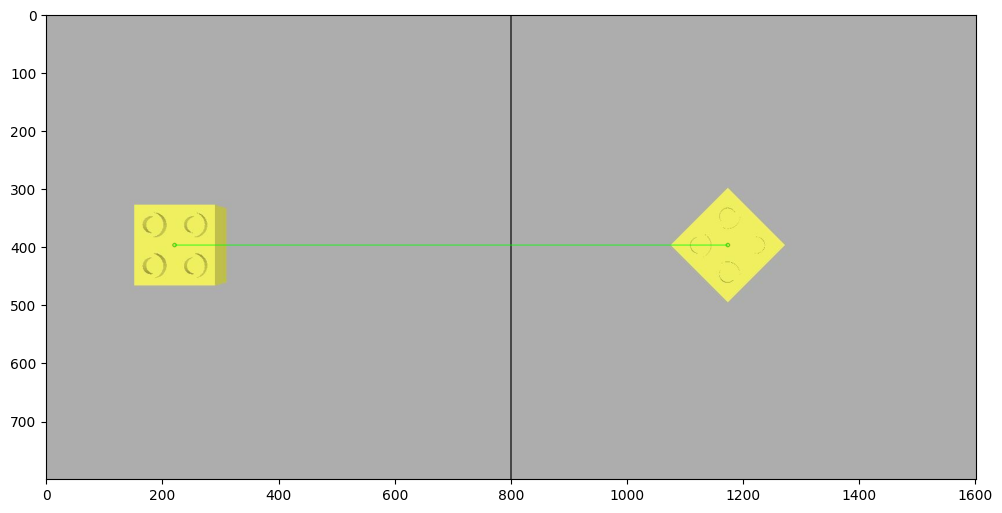
\includegraphics[width=\textwidth]{figures/ideal_centre-of-mass.png}
    \caption{Centre of mass matching}
    \label{fig:centre-of-mass}
\end{figure}

However, note that while a single point is enough to compute the translation offset between the object in different scenes, it is not sufficient to compute the orientation offset. By reducing the object in the image to a single point, we have estimated its position, but have no information about its orientation. This is a problem for us since we want the system to be robust to not only moving the object, but also rotating it. Some objects may behave very differently in different orientations if they do not have rotational symmetry. As such we need a way to estimate the orientation of the object in both images.\\

In order to achieve this we cannot reduce the object to a single central point, but we can reduce it to a collection of points. Having multiple points which match in the two images can allow us to identify if a translation or rotation have occurred. \reffig{fig:ideal-matches} shows how an ideal set of matches allows us to infer both a translation and rotation between the object in the images. In this case we can see the block needs to move to the right of the frame, but now also needs to rotate approximately 45$\degrees$ anticlockwise (a positive rotation according to the right hand rule) about the vertical axis.

\begin{figure}[h]
    \centering
    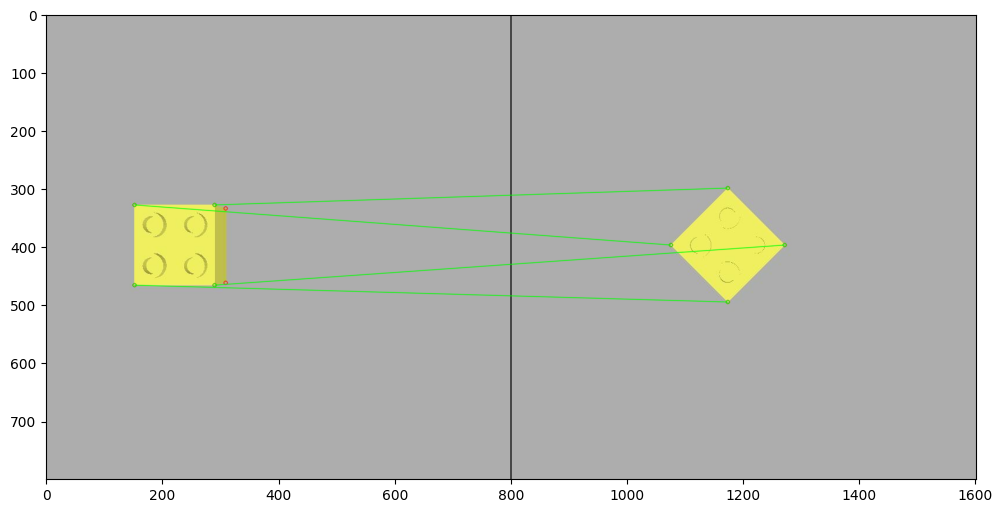
\includegraphics[width=\textwidth]{figures/ideal_matches.png}
    \caption{Ideal keypoint matching}
    \label{fig:ideal-matches}
\end{figure}

Note that this is only one way the keypoints could be matched. \reffig{fig:ideal-matches-inv} shows another way we may choose to match the keypoints. In this case the live object should move to the right and rotate approximately 45$\degrees$ clockwise (a negative rotation according to the right hand rule) about the vertical axis, in order to align with the demonstration object. While having multiple possible ways to match the keypoints may seem like a problem, this is merely a consequence of the object in question having rotational symmetry. It does not matter which way we rotate the object, because it will behave the same, whichever side we are facing, and each side is indistinguishable from each other. As such, for our purposes it would not matter which matching and subsequent transformation we chose, since in either case the object is aligned to the demonstration image. In practice this situation would not likely occur, since we will have many more keypoints, and the keypoints will very likely not be evenly spaced as in this ideal example.

\begin{figure}[h]
    \centering
    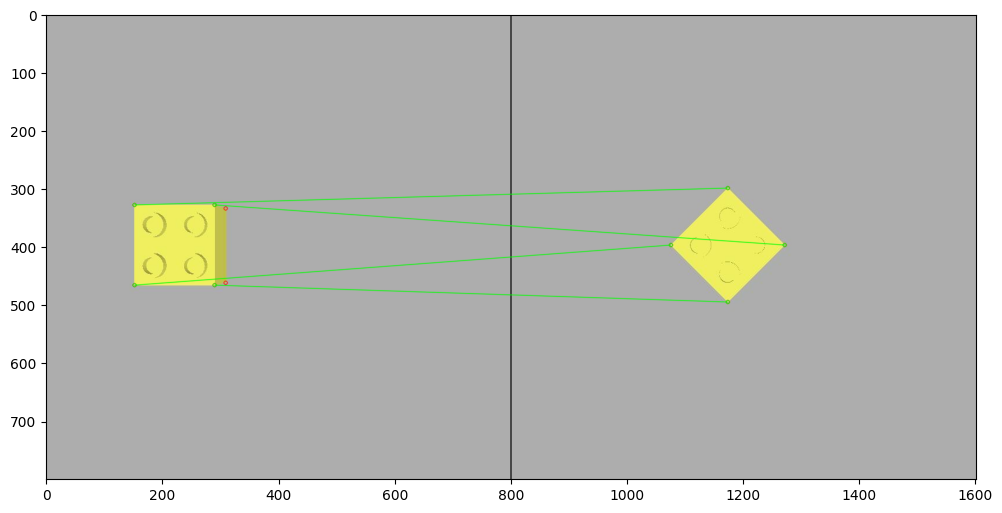
\includegraphics[width=\textwidth]{figures/ideal_matches_inv.png}
    \caption{Alternative ideal keypoint matching}
    \label{fig:ideal-matches-inv}
\end{figure}

We can also see that in both figures, the live image contains two additional keypoints marked in red. These keypoints could not be matched to any in the demonstration image so are ignored when calculating the translation and rotation to align the objects. In this case it is because these keypoints become occluded when we view the object in the demonstration image.\\

These figures are designed to give an intuition for how we can use keypoints to find the desired end effector offset. In these figures we have considered ideal keypoints where the keypoints are extracted on useful points of the image, namely the object corners, and where the matching is perfect with no mistakes. These keypoints have been placed by a human for the purposes of demonstration. Obviously for the complete system we want the keypoint extraction and matching to be automated. How we achieve this will be explored next.

%TODO undecided whether this or kabsch section should come first
\subsection{Automated keypoint extraction and matching}
\label{subsec:keypoint-algos}
Keypoint extraction is a popular and well studied problem in the field of computer vision. As such we have many options at our disposal. Our goal is to identify the pixels where the image changes significantly. These may be where 
%TODO mention experiments in evaluation section which tells us the best algorithm for extraction and matching

\subsection{Calculating end effector offset}
\label{subsec:kabsch}
Now that we have a list of matched keypoint pairs, we can begin to calculate the offset between the object in the live and demonstration image. Fortunately there exists an algorithm for computing the translation, rotation and scaling, which best maps a set of points onto another set of points. This algorithm is called the \socalled{Kabsch-Umeyama algorithm}. The algorithm takes in two sets of points, a reference set P, and a test set Q. It computes a translation t, a rotation matrix R and a scale factor s, such that when these transformations are applied to Q, yielding Q', the root mean squared distance between P and Q' is minimized. For our purposes we make a number of important modifications to the original algorithm to better fit our 

As mentioned above, we decide to convert all keypoints to world coordinates first. By doing this we can more easily include the depth information of the image. Additionally, this will result in the translation computed already being in world coordinate units, meaning no further calculation is needed to calculate how far to move the end effector.\\

...
The first step of the algorithm will look familiar to something we tried in \refsubsec{subsec:keypoints}. The first step is to compute the centroids of the two sets of points. This is just the average position of all the points in the set. This acts like the centre of mass of the point set. With sufficiently many and well spaced keypoints in our set, this centre of mass will be approximately equal to the centre of mass we computed earlier by considering all pixels of the object. As we discussed earlier, the centre of mass of the points will be enough to compute the translation between the two sets.
$$\overline{p} = \frac{1}{|P|}\sum_{p \in P}p \longspace \overline{q} = \frac{1}{|Q|}\sum_{q \in Q}q$$
The next step is to re-centre the points so that the centre of mass is on the origin. It is therefore clear that to achieve this we will 
... covariance shit
After 

%TODO mention experiments for how it behaves with noise applied to ideal matches.
% create random unit vector, and random magnitude of noise. This way we can ensure noise is in a tight window. So we can say this is how it perfromed with 1-5 pixels noise, 5-10. Better than 1-5 and 1-10.


%keypoint extraction - diagrams to show how we extract keypoints, what sort of parts are keypoints due to change in derivative.
%  - SIFT vs BRIEF/ORB
% 
% Keypoint matching - the different distance metrics for SIFT and ORB.
%  diagrams for how matching can help us identify translations and rotations, ideal matches
% GMS (Do more research as to how it works) and how we refine matches into better matches for our purposes
% calculating transformation from matches (not sure where this section should go. Could move higher up to motivate why we extract keypoints at all)
% Go through the equations, cite Kabsch algorithm, explain why we compute translation without R since we consider rotation as spinning in place and so translation is just the offset in centroids.

\newpage




\section{Decomposing the reward function}
\label{sec:reward-function}
At this point we have a system which can transform a trajectory from the demonstration environment to a new unseen environment containing the same object. Our goal now is to extend this system to transform the trajectory into an environment containing different objects. The current system will select the demonstration whose context image matches the current scene most closely. This allows it to select the correct demonstration whose context image contains the target object in the current scene. However, this naturally extends to unseen objects since the similarity metric used will still compare the current scene to all context images and select the most similar. We can expect the similarity between the embeddings of the two images to be greatest when they contain the same objects, however if no such demonstration exists on this specific object, we can still select whichever demonstration is closest. Since we directly compare not the images themselves, but the image embeddings from the vision transformer, this translates to selecting the image with the object whose dino feature points are most similar. In essence, the object which behaves most similarly to the current scene object. Therefore we can expect the system to already choose the demonstration which is closest to working with this new object. For example if the demonstration was to pick up a can, it is likely that when faced with a bottle in the current scene that the system would select the can demonstration. This is because the objects appear similar as they are both cylindrical items, and the robot would have to interact with them in similar ways, by grasping around the cylinder. As such we can conclude that the can demonstration is the closest one to working with this new object.
%TODO check this paragraph isnt too rambly
%also should this be at the start of this section or the end of the prev one?
% I think the prev one

The hope would be that these two objects are similar enough that the same demonstration would already be able to successfully complete the task on this new object.

%TODO the later stuff is no longer relevant but the above paragraph could still be good to talk about. Just slightly reword stuff to sound like this is a happy bonus rather than the original focus


Designing the reward function to score how good an executed trajectory was will be very complicated since we need to encode so many intuitive notions into rigorous mathematics. For example, if the trajectory ends in some state $s$ then we want to ask \speech{Does this state represent some task having been completed?} This is very hard to do since the task could be anything, and we have little prior knowledge of what the robot was intending to achieve. Additionally for each state along the trajectory we would also ask questions of \speech{Is this state interesting?} \speech{Is this state unlike states we have seen before?} \speech{Was this state what we expected to happen by completing these actions, or was the outcome surprising?} We need ways to mathematically encode each of these questions from the series of state, action pairs along the robot's trajectory. We will also need to weight the relative importance between each aspect of the reward function.\\

We start by considering how to categorise the above questions. Particularly we may notice that the question of \speech{Was a task completed?} concerns primarily the final state of the trajectory. It wants to know information external to the trajectory itself, particularly, was a meaningful task accomplished by this trajectory. The other questions however, ask about the inherent properties of the trajectory, were the states involved interesting, novel or surprising? These two different categories are called extrinsic and intrinsic rewards respectively. Our final reward function will be some combination of both types.\\
\textbf{\textit{Extrinsic rewards}} motivate the agent to learn to complete a specific task. The specifics of the trajectory itself are unimportant, if the task has been completed then a high reward is given. The problem with extrinsic rewards is that they are by definition, dependent on the task at hand. This requires us to define a reward function for each task. This flies in direct opposition to the goal of this paper which is to produce an agent which can learn to perform new tasks which were unseen in the demonstrations. One potential solution is to use external rewards. This strategy does not have an analytically defined reward function. Instead we ask a human for input to decide the reward the robot gets for this trajectory. This could be on a scale from 0 to 1 where 1 is perfectly completing the task. This system has promise because despite requiring human input, it offloads the complex intuition required to properly score the trajectory. Specifically because the agent is attempting to solve new tasks, the human is able to infer what the robot was going for, and grade accordingly. If the robot manages to pick up an object, we can be reasonably sure this was the goal of the task, and it has therefore been completed. This high level reasoning about what the task was and subsequently has it been achieved, would be very difficult for a computer system to evaluate.\\
\textbf{\textit{Intrinsic rewards}} in contrast, motivate the agent to produce better trajectories. For example trajectories which are different from other previously seen trajectories. These rewards are concerned only by the internal properties of the trajectories and do not care about the impact this trajectory has on the external environment.




% \chapter{Project Plan}
% \label{chap:plan}


% \section{Technical Progress}
% Technical progress so far has been limited while a focus has been put on research and writing this interim report. The main implementation achievements thus far have been on important utilities for later in the project. In particular downloading the necessary files and initialising the simulator is obviously key to the success of this project and so was completed as a priority.\\

% Following this, a utility program was created for generating demonstration trajectories. As discussed in Chapter \ref{chap:background}, this project aims to use imitation learning to teach the agent an initial collection of skills. As such, a program to streamline the collection of demonstrations for the imitation learning will be a useful asset throughout this project.\\

% This program allows for individual joint control by selecting and moving joints independently. Once the arm is positioned in the correct pose, the user can save the current pose as a key frame of the trajectory. From here they can move the arm again and save the next key frame. If a mistake is made, the user can revert the robot arm to the last saved key frame.\\
% The trajectory is stored as a list of joint poses. Each element of the trajectory is a key frame robot state. The key frame stores the joint angles of the robot's 11 joints (although not all joints are actuated so a small number of these 11 joints are permanently fixed at 0 radians).

% The program is written to interface with a video game controller, so that the user can control joint angles using an analogue input method such as the joysticks. This makes the program slightly more user friendly, as moving the joystick only slightly will move the joint very slowly and so allows for finer control.\\
% In addition to controlling joint poses, the program allows for camera rotation and zooming to better see the full robot pose, and colour codes the current joint the user is controlling in the wire-frame view, visible in Figure \ref{fig:arm-wire}.



% \section{Future Plans}
% The project plan can be broken into small short term goals which will be built upon, and longer term goals which constitute the bulk of the project. This project aims to complete the goals by the deadline shown:

% \subsection*{End of January 2024}
% Since very little time remains before the end of January, a very small goal of further improvements to the trajectory generating utility program is set. The program should be modified to allow for a second control mode. Instead of individually controlling each joint angle, it should be possible to control the 3D position of the end effector, and use inverse kinematics to calculate the joint angles from this position. The two control modes should work with each other and be able to switch between them while using the program.

% \subsection*{End of February 2024}
% By the end of February the first stage of the learning algorithm should be in place. This is implementing the one-shot imitation learning algorithm as described by  N. Di Palo, and
% E. Johns \cite{one-shot-imitation}. This first part of the algorithm will allow us to provide the agent with an initial set of skills, from which it can explore and learn more.

% \subsection*{End of March 2024}
% By the end of March this project hopes to implement the next step of the algorithm which involves the noise based exploration of the nearby state space. The agent will select a known skill trajectory and try adding noise to it to investigate what happens. The idea being that the agent selects the most similar skill from its repertoire, and so small amounts of learned noise will be sufficient for a task that nearly succeeded. For example, starting with the trajectory to pick up a water bottle, the agent may be able to learn how to pick up a can by simply augmenting the known trajectory. The action of picking up both objects are very similar, but the robot may need to grab lower on the can since it is shorter than the bottle. This slight deviation will be captured by the noise. Once an amount of noise is learned which is successful at completing the new task, the original trajectory and noise can be saved together as a new skill.\\
% This is a large part of the algorithm and March also contains end of term exams, reducing the amount of time available for the project in the final weeks of March. As such this is a soft deadline, and we anticipate the need for this implementation point to bleed into the next month's milestones.

% \subsection*{End of April 2024}
% By the end of April this project aims to be at the final implementation step. This will include the \socalled{curiosity based reward function} to encourage exploration of interesting or uncertain parts of the state space, which will hopefully lead to more unique and successful skills being learned.\\
% The other feature we plan to implement by April is the human based skill descriptor system. As discussed in Chapter \ref{chap:introduction}, this would allow the robot to demonstrate its self-taught skills where the human can provide context and a name to this skill. This can then be used in a deployed setting with a language model to give the agent orders to complete tasks based on its learned skills.

% \subsection*{End of May 2024}
% The month of May is intended to be used to run larger scale experiments and fine tune the algorithm. By this point the bulk of the implementation should be complete and this project should be looking to collect lots of results, and potentially deploy the agent to a physical robot arm. The transition from simulation to real world will undoubtedly bring challenges through the inaccuracies of real life such as joint frictions or differences in the simulated and true masses of objects and the robot arm segments. These small inaccuracies of the simulation may lead to compounding problems which affect the success rate of the agent. If this is the case then further tuning will be considered to improve the agent again.

% \subsection*{17th June 2024}
% The month of June is reserved for finishing and polishing the final report. By this deadline the project, experiments and accompanying report should all be completed.
\chapter{Evaluation}
\label{chap:evaluation}
In this section, we evaluate the performance of our algorithm against a custom test suite. Our evaluation consists of two main tests designed to assess different aspects of the algorithm.\\
In the first test we examine how well our modified Kabsch-Umeyama algorithm handles varying levels of noise helping us understand its stability and robustness to perform well even in noisy environments.\\
The second test compares different key point matching algorithms by using them in a full run of the system and measuring their performance under identical environmental conditions. Following this test we will determine the best algorithm for use in our project, finalising the implementation design.

\section{Sensitivity to noise}
%evaluate how the kabsch algorithm performs with noise applied to ideal keypoints
In this test we want to understand how robust our modified Kabsch-Umeyama algorithm is to noise in the coordinates it receives. The hope is that small deviations to the coordinate inputs produce very small changes in the output translation and rotation matrix. If this is the case then the algorithm is robust to noise, and is more likely to produce good results when used in our system.\\

%TODO should really make a bigger suite, update number if we do
In order to conduct this test we create a test suite of 5 diverse objects and an accompanying demonstration for each one. We then manually mark an ideal set of key points in the demonstration image. These key points are recorded as a list of (x,y) pixel coordinate pairs. We also make sure to record the position and orientation of the object in the demonstration.
We then place this same object in a different pose in the environment and save the live image from the robot in this case. Again making sure to note down the position and orientation of the object in this new scene. We then again manually mark the same key points but in this new image. It is important that we mark corresponding key points, so if in the demonstration we marked the corners of a cube, we must also mark the corners in the live image. The pixel location of these corners will just have moved. \reftab{tab:test-suite} shows the transformation between the demonstration and live object pose. We also disclose how many keypoints were manually marked for each object.\\

\begin{table}[h!t]
    \begin{adjustbox}{center}
        \begin{tabular}{| V{5cm} || c | c | c |}
            \hline
            \rowcolor{lightgray!25}
            Object & Translation applied & Rotation applied & Number of key points \\
            \hline
            Lego & [-0.1, 0.05, 0] & [0, 0, $\frac{\pi}{3}$] & 4\\
            \hline
            Mug & [0, 0.05, 0] & [0, 0, $\frac{\pi}{6}$] & 16\\
            \hline
            Ball & [] & [] & \\
            \hline
            Block & [0.1, 0.15, 0] & [0, 0, $-\frac{\pi}{6}$] & \\
            \hline
            Domino & [0.05, 0.07, 0] & [0, 0, -$\frac{\pi}{4}$] & \\
            \hline
        \end{tabular}
    \end{adjustbox}
    \caption{The true transformation between demo and live for each object in test suite}
    \label{tab:test-suite}  
    \end{table}

Now we can pass the manually marked key points in the demonstration and live image to our modified Kabsch-Umeyama algroithm. This should output the exact translation and rotation between the object from the demonstration to the live scene, within a small tolerance of floating point accuracy. The purpose of using human provided, ground truth key points is to control any additional noise in the test. If we used our keypoint matching algorithm then it would be unclear how much error came from our randomly added noise, or from mismatches in the key point algorithm. As such we gain clearer results by using our ground truth key points.\\

With the method defined, we now add some noise to the ideal key points before passing them to the algorithm. We wish to compare how far the new output deviates from the true output when the noise is added. Since we add random noise, we conduct multiple runs and compute the average.\\

In this first set of tests the noise added is calculated as a random 3D unit vector multiplied by some random magnitude. The magnitude will be drawn from a uniform distribution, in the range $[a,b]$. Here $a$ and $b$ are used to control the upper and lower bounds on how much noise can be added. This allows us to perform multiple tests and compare the effects of increasingly large deviations.\\
When computing the random 3D unit vector, we take care to use an \speech{equal area projection of the sphere onto a cylinder} \cite{uniform-3d-vector, cylinder-proj, random-vector}. This allows us to choose a point uniformly from the unit sphere, without experiencing a bunching of points at the poles. This random noise is applied to the world coordinates after they have been computed from the pixel coordinates. This gives us a solid grasp as to just how much noise can be present before the algorithm produces unsatisfactory results.\\

In the second set of tests we change how we apply the random noise to better emulate our system. Since the pixel to world coordinate calculations use the exact view matrix of the camera, the only errors in this part of the system are the result of very small floating point inaccuracies. The source of the error will be predominantly a result of the key point matching. As such in this second round of tests, we add noise to the pixel coordinates of the key points, before converting them to world coordinates. This is more representative of the type of error we will encounter in this system, and so proves a more reliable result.
% table of results

\section{Comparison of keypoint algorithms}
%evaluate SIFT vs ORB vs SIFT with GMS vs ORB with GMS vs our new one if we have time to make it
We discussed in \refsubsec{subsec:keypoint-algos} that there are multiple different algorithms we could use for our system. Any algorithm which can extract and match keypoints can be used. In this section we analyse a few different aproaches 

%OLD STUFF
%We will evaluate the success of this project by analysing the proportion of tasks the agent is able to successfully complete. We will compare these results to similar approaches in the field \cite{one-shot-imitation, one-shot-pose-estimate}.
%As described in these papers, the methods used for one-shot imitation learning generalise well to completing the same tasks with different objects. For example picking up a different water bottle to the one in the demonstration. We also know that they generalise to different environment setups, robust to rotations and translations of the objects in the scene. We hope that this project will allow the agent to generalise even further beyond, to skills which differ conceptually to those shown in the demonstrations. We hope that this extra level of generalisability will provide improved success rate metrics on unseen tasks compared to the state of the art current solutions. The existing solutions appear to limit their unseen test set to the same categories of task as their training set, just with new unseen objects. We hope that in this project we can expand this test set to a much more wide spread of potential tasks, and still see high success rates in the testing phase.\\

%In addition to evaluating our algorithm under ideal conditions we would like to investigate how robust it is to its starting configuration. Due to the design of the learning algorithm, it is likely that the ability to learn new skills will be affected by the quality of initial demonstrations. We hypothesise that an agent given 10 unique and diverse demonstrations, will perform better in unseen task completion, than an agent trained with 10 demonstrations which all just involve picking up similar objects. This is because the algorithm as proposed, learns through augmenting existing demonstrations with noise. As such, the skills the agent will learn are likely to conceptually branch off of an existing skill. If the initial skill set is very diverse, then this allows the agent to search a wider portion of the space of all trajectories. Comparatively, if the initial skills are all very similar, then the agent has a harder time searching wide in the search space since it can only save a new skill by augmenting existing skills. A simplified example of this is shown in Figure \ref{fig:trajectory-space} with a 2D search space. In practice the space of all trajectories is far more than 2 dimensions. This makes having diverse initial skills which cover the search space as best as possible even more important since there is far more for the agent to search.

% \begin{figure}[ht]
%     \centering
%     \begin{subfigure}[b]{0.45\textwidth}
%         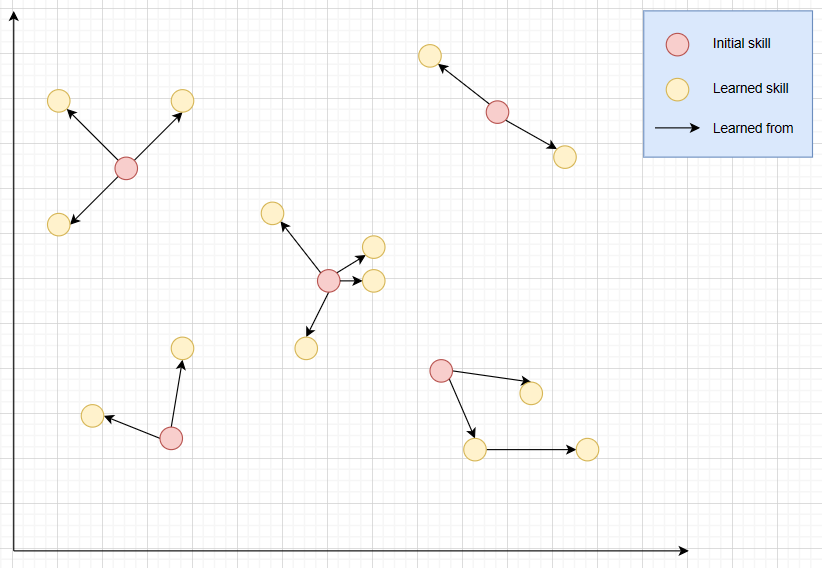
\includegraphics[width=\textwidth]{figures/graph_spread.PNG}
%         \caption{Diverse initial skill set}
%     \end{subfigure}
%     \hfill
%     \begin{subfigure}[b]{0.45\textwidth}
%         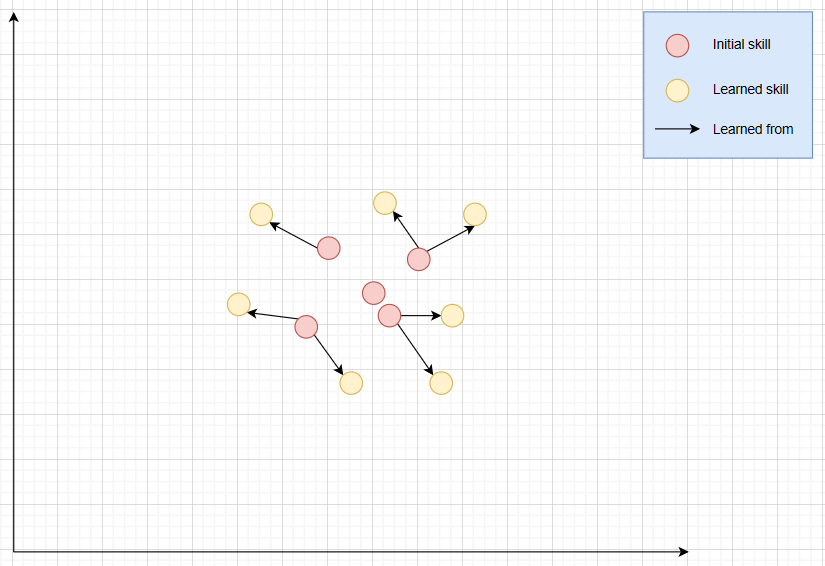
\includegraphics[width=\textwidth]{figures/graph_narrow.PNG}
%         \caption{Narrow initial skill set.}
%     \end{subfigure}
%     \caption{Simplified diagram of trajectory search space.}
%     \label{fig:trajectory-space}
% \end{figure}

% In Figure \ref{fig:trajectory-space} nodes of the graph represent the trajectories which succeed in performing some task and are saved as a skill. Edges represent that the child skill was learned by augmenting the parent skill. Nodes with no parent are the initial skill set, coloured red.
\chapter{Conclusion}
\label{chap:conclusion}

In this paper we have demonstrated the use of a One-shot Imitation Learning framework, which is capable of running with no GPU requirements. Furthermore, the RAM usage is remarkeably low, peaking at .

\bibliographystyle{unsrtnat} %alpha
\bibliography{references}

\appendix
\chapter{Null space inverse kinematics}
\label{apx:null-space}
As discussed in \refsec{sec:trajectories}, inverse kinematics will be an underdetermined system if the number of controllable joints exceeds the degrees of freedom of the desired end effector pose. This has the effect of having infinitely many, all equally valid robot poses which achieve the desired end effector position. However, this is only in theory. Consider \reffig{fig:ik-invalid}. Here we can see that the solution requires two of the arm links to intersect. While this is fine in theory and does constitute a solution to the IK system, in the real world the links of the robot arm are not infinitely thin line segments, they are physical parts with thickness. If this robot was in the real world this would require parts of the robot to pass through each other. This is obviously impossible in a real situation.

\begin{figure}[h]
    \centering
    \begin{subfigure}[b]{0.45\textwidth}
        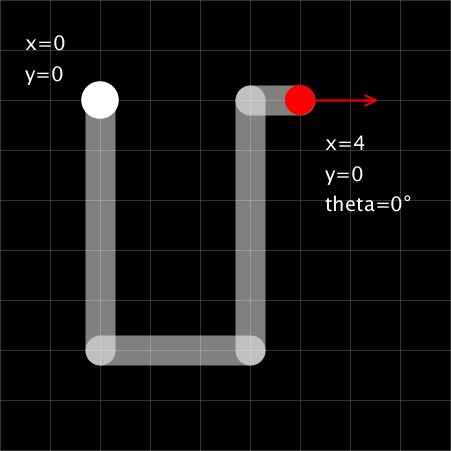
\includegraphics[width=\textwidth]{figures/ik-valid.png}
        \caption{A valid IK solution}
        \label{fig:ik-valid}
    \end{subfigure}
    \hfill
    \begin{subfigure}[b]{0.45\textwidth}
        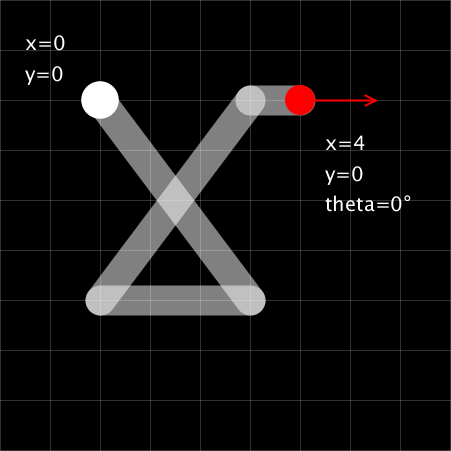
\includegraphics[width=\textwidth]{figures/ik-invalid.png}
        \caption{An invalid IK solution}
        \label{fig:ik-invalid}
    \end{subfigure}
    \caption{Not all IK solutions may be valid}
    \label{fig:ik-null-space}
\end{figure}

Fortunately for us, we saw that by having additional degrees of freedom, we can generate infinitely many solutions to the IK system. This means we could prune these invalid solutions by adding additional constraints. While it is possible this could make all solutions invalid, this is both unlikely and necessary. These invalid solutions remain because the current IK system does not perfectly capture our real world restrictions. If all solutions are removed by our additional constraints, then this simply means the desired end effector pose was not possible in a real world system.\\

There are two main ...



\chapter{Evaluation Test Suite}
\label{apx:test-suite}

This appendix details specifics about the test suite used in \refchap{chap:evaluation}.\\

\begin{figure}[h]
    \centering
    \begin{subfigure}[b]{0.49\textwidth}
        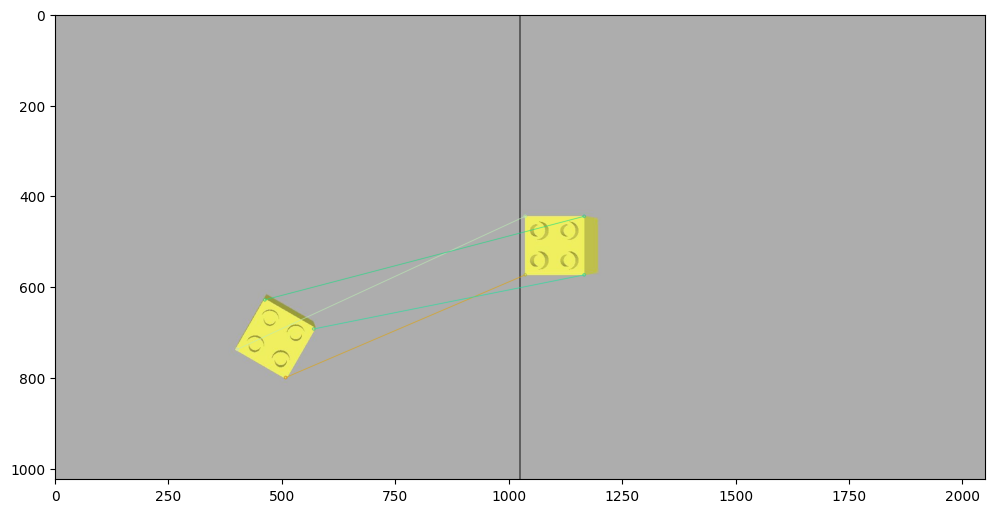
\includegraphics[width=\textwidth]{figures/matchLego.png}
        \caption{Lego object}
    \end{subfigure}
    \hfill
    \begin{subfigure}[b]{0.49\textwidth}
        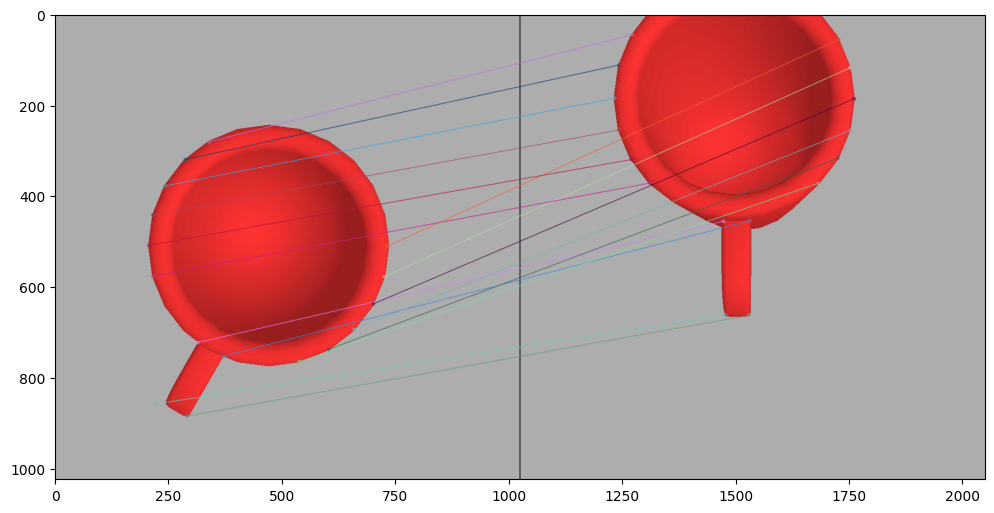
\includegraphics[width=\textwidth]{figures/matchMug.png}
        \caption{Mug object}
    \end{subfigure}

    \begin{subfigure}[b]{0.49\textwidth}
        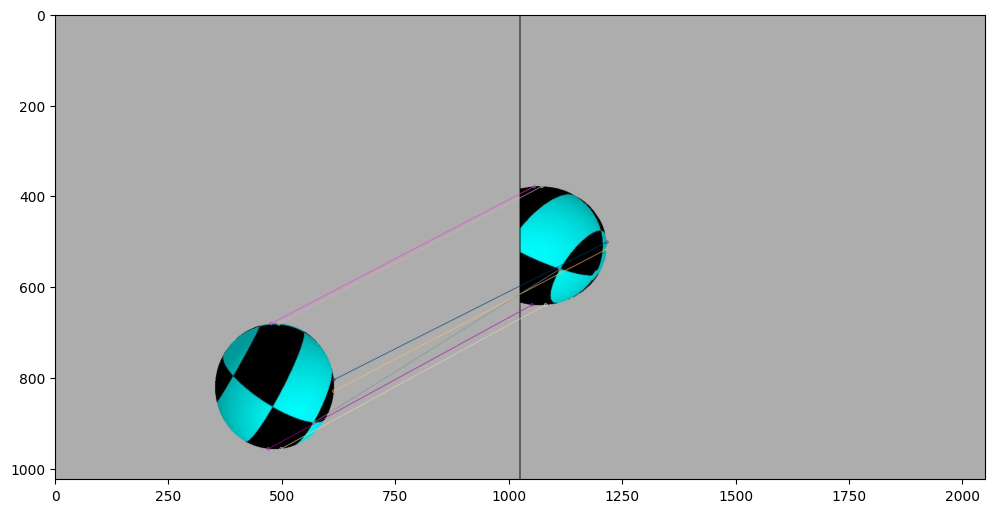
\includegraphics[width=\textwidth]{figures/matchBall.png}
        \caption{Ball object}
    \end{subfigure}
    \hfill
    \begin{subfigure}[b]{0.49\textwidth}
        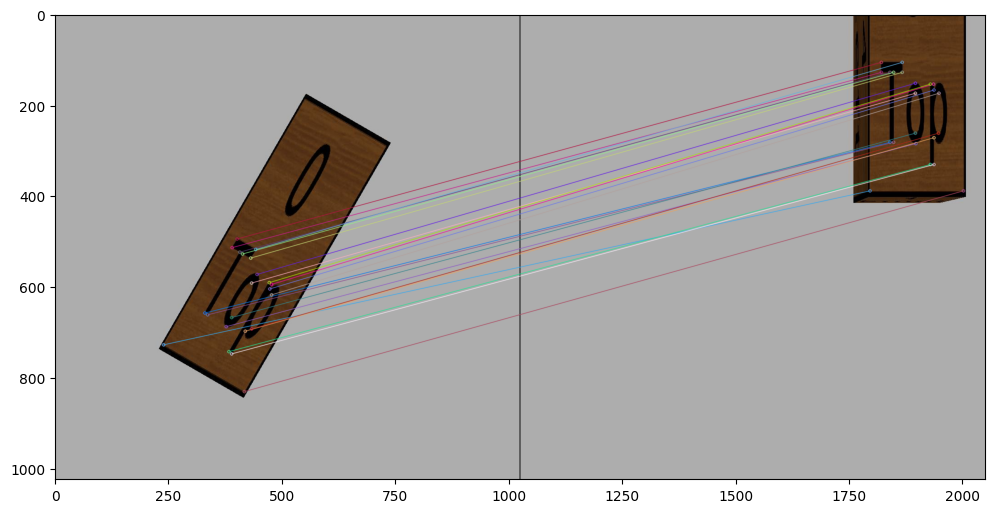
\includegraphics[width=\textwidth]{figures/matchJenga.png}
        \caption{Jenga block object}
    \end{subfigure}
    
    \begin{subfigure}[b]{0.49\textwidth}
        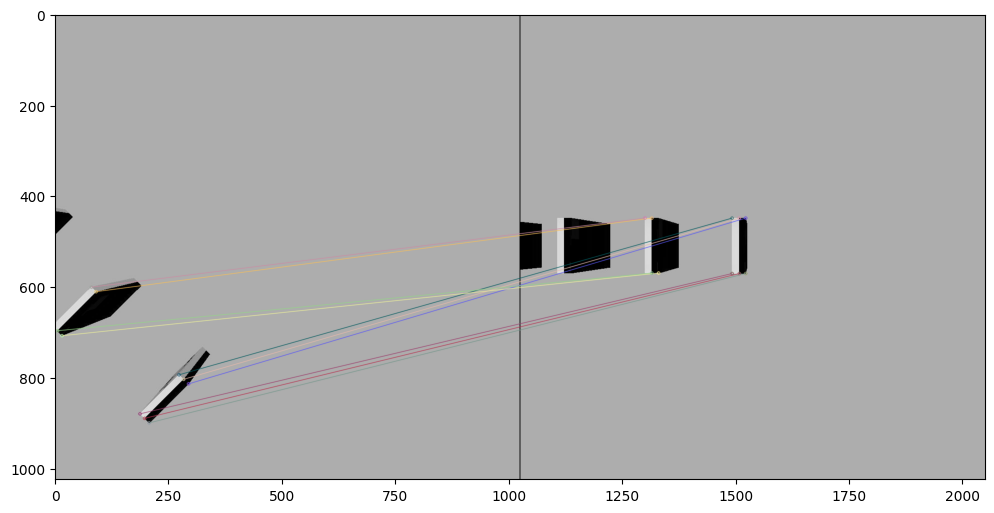
\includegraphics[width=\textwidth]{figures/matchDominoes.png}
        \caption{Domino objects}
    \end{subfigure}
    \caption{Live and demonstration images used in test suite, with human marked keypoint matches}
    \label{fig:testImages}
\end{figure}


By analysing these images we can understand why some of the objects are more sensitive to noise, as explored in \refsec{sec:noise-test}.
%TODO include observations from second test. ie which objects are forgiving, which fail more tests (i bet sphere)

\subsubsection{Lego object}
In this object the keypoints are marked as the 4 corners. It is very easy to identify these even when the object was rotated. This explains why this object had the lowest systematic error (as discussed in \refsec{sec:noise-test}) because the human error was very close to 0.

\subsubsection{Mug object}
In this object the keypoints are marked at even intervals around the mug, as well as the corners of the handle. However, in the demonstration image, the top of the mug is out of frame. This reduces how many keypoints we can identify. The circular nature of this object makes placing keypoints in the exact correct position more challenging.

\subsubsection{Ball Object}
This object is surprisingly difficult to mark keypoints given it is a perfect sphere. As such keypoints move in difficult to predict ways for a human keypoint matcher. Furthermore, the 

\subsubsection{Jenga block object}
This object experienced the largest amount of systematic error by a large margin in \refsec{sec:noise-test}. Initially one might think that it should be easy to identify keypoints. Like with the Lego object, we may try to mark the corners of the block. However, in the demonstration image the top of the block is out of frame. This is deliberate to make the test more challenging for the system. As a result we can only mark the bottom two corners as keypoints. Instead we match identifiable points of the text on the object. This allows us to manually identify far more keypoints, the most of any object at 22. However, these keypoints are prone to a large amount of human error, since the text does not form clean lines in the bitmap image. As such in the rotated live image, it can be difficult to locate the correct pixel. The human error across all the keypoints accumulates, leading to the largest systematic error of any object in the test suite.

\subsubsection{Dominoes}
This object is interesting because it is actually not a single object but multiple. The rotation applied in \reftab{tab:test-suite} is not applied about the centre like other objects. The line is rotated about the first domino. This presents some challenges for the robot since in order to knock over the domino line successfully it needs to rotate the vector it approaches at, unlike most objects where the angle of approach does not matter, provided the end effector is spun to the correct angle.\\

In this test we can only identify a small number of keypoints since the majority of the domino line is out if frame.


\chapter{Additional Evaluation Figures}
\label{apx:more-figures}

This appendix contains additional figures from the evaluation in \refchap{chap:evaluation}. These figures contain additional or alternative information which can give further insight into the conclusions drawn in that section. However, they are relegated to this appendix due to the page limit of this report, and the belief that the information displayed is less crucial than the figures included in \refchap{chap:evaluation}.\\


\end{document}